\documentclass[12pt]{article}

%packages
%\usepackage{latexsym}
\usepackage{graphicx}
\usepackage{color}
\usepackage{amsmath}
\usepackage{dsfont}
\usepackage{placeins}
\usepackage{amssymb}
\usepackage{wasysym}
\usepackage{abstract}
\usepackage{hyperref}
\usepackage{etoolbox}
\usepackage{datetime}
\usepackage{xcolor}
\usepackage{alphalph}
\usepackage{bm}
\settimeformat{ampmtime}

%\usepackage{pstricks,pst-node,pst-tree}

%\usepackage{algpseudocode}
%\usepackage{amsthm}
%\usepackage{hyperref}
%\usepackage{mathrsfs}
%\usepackage{amsfonts}
%\usepackage{bbding}
%\usepackage{listings}
%\usepackage{appendix}
\usepackage[margin=1in]{geometry}
%\geometry{papersize={8.5in,11in},total={6.5in,9in}}
%\usepackage{cancel}
%\usepackage{algorithmic, algorithm}

\makeatletter
\def\maxwidth{ %
  \ifdim\Gin@nat@width>\linewidth
    \linewidth
  \else
    \Gin@nat@width
  \fi
}
\makeatother

\definecolor{fgcolor}{rgb}{0.345, 0.345, 0.345}
\newcommand{\hlnum}[1]{\textcolor[rgb]{0.686,0.059,0.569}{#1}}%
\newcommand{\hlstr}[1]{\textcolor[rgb]{0.192,0.494,0.8}{#1}}%
\newcommand{\hlcom}[1]{\textcolor[rgb]{0.678,0.584,0.686}{\textit{#1}}}%
\newcommand{\hlopt}[1]{\textcolor[rgb]{0,0,0}{#1}}%
\newcommand{\hlstd}[1]{\textcolor[rgb]{0.345,0.345,0.345}{#1}}%
\newcommand{\hlkwa}[1]{\textcolor[rgb]{0.161,0.373,0.58}{\textbf{#1}}}%
\newcommand{\hlkwb}[1]{\textcolor[rgb]{0.69,0.353,0.396}{#1}}%
\newcommand{\hlkwc}[1]{\textcolor[rgb]{0.333,0.667,0.333}{#1}}%
\newcommand{\hlkwd}[1]{\textcolor[rgb]{0.737,0.353,0.396}{\textbf{#1}}}%

\usepackage{framed}
\makeatletter
\newenvironment{kframe}{%
 \def\at@end@of@kframe{}%
 \ifinner\ifhmode%
  \def\at@end@of@kframe{\end{minipage}}%
  \begin{minipage}{\columnwidth}%
 \fi\fi%
 \def\FrameCommand##1{\hskip\@totalleftmargin \hskip-\fboxsep
 \colorbox{shadecolor}{##1}\hskip-\fboxsep
     % There is no \\@totalrightmargin, so:
     \hskip-\linewidth \hskip-\@totalleftmargin \hskip\columnwidth}%
 \MakeFramed {\advance\hsize-\width
   \@totalleftmargin\z@ \linewidth\hsize
   \@setminipage}}%
 {\par\unskip\endMakeFramed%
 \at@end@of@kframe}
\makeatother

\definecolor{shadecolor}{rgb}{.77, .77, .77}
\definecolor{messagecolor}{rgb}{0, 0, 0}
\definecolor{warningcolor}{rgb}{1, 0, 1}
\definecolor{errorcolor}{rgb}{1, 0, 0}
\newenvironment{knitrout}{}{} % an empty environment to be redefined in TeX

\usepackage{alltt}
\usepackage[T1]{fontenc}

\newcommand{\qu}[1]{``#1''}
\newcounter{probnum}
\setcounter{probnum}{1}

%create definition to allow local margin changes
\def\changemargin#1#2{\list{}{\rightmargin#2\leftmargin#1}\item[]}
\let\endchangemargin=\endlist 

%allow equations to span multiple pages
\allowdisplaybreaks

%define colors and color typesetting conveniences
\definecolor{gray}{rgb}{0.5,0.5,0.5}
\definecolor{black}{rgb}{0,0,0}
\definecolor{white}{rgb}{1,1,1}
\definecolor{blue}{rgb}{0.5,0.5,1}
\newcommand{\inblue}[1]{\color{blue}#1 \color{black}}
\definecolor{green}{rgb}{0.133,0.545,0.133}
\newcommand{\ingreen}[1]{\color{green}#1 \color{black}}
\definecolor{yellow}{rgb}{1,1,0}
\newcommand{\inyellow}[1]{\color{yellow}#1 \color{black}}
\definecolor{orange}{rgb}{0.9,0.649,0}
\newcommand{\inorange}[1]{\color{orange}#1 \color{black}}
\definecolor{red}{rgb}{1,0.133,0.133}
\newcommand{\inred}[1]{\color{red}#1 \color{black}}
\definecolor{purple}{rgb}{0.58,0,0.827}
\newcommand{\inpurple}[1]{\color{purple}#1 \color{black}}
\definecolor{backgcode}{rgb}{0.97,0.97,0.8}
\definecolor{Brown}{cmyk}{0,0.81,1,0.60}
\definecolor{OliveGreen}{cmyk}{0.64,0,0.95,0.40}
\definecolor{CadetBlue}{cmyk}{0.62,0.57,0.23,0}

%define new math operators
\DeclareMathOperator*{\argmax}{arg\,max~}
\DeclareMathOperator*{\argmin}{arg\,min~}
\DeclareMathOperator*{\argsup}{arg\,sup~}
\DeclareMathOperator*{\arginf}{arg\,inf~}
\DeclareMathOperator*{\convolution}{\text{\Huge{$\ast$}}}
\newcommand{\infconv}[2]{\convolution^\infty_{#1 = 1} #2}
%true functions

%%%% GENERAL SHORTCUTS

%shortcuts for pure typesetting conveniences
\newcommand{\bv}[1]{\boldsymbol{#1}}

%shortcuts for compound constants
\newcommand{\BetaDistrConst}{\dfrac{\Gamma(\alpha + \beta)}{\Gamma(\alpha)\Gamma(\beta)}}
\newcommand{\NormDistrConst}{\dfrac{1}{\sqrt{2\pi\sigma^2}}}

%shortcuts for conventional symbols
\newcommand{\tsq}{\tau^2}
\newcommand{\tsqh}{\hat{\tau}^2}
\newcommand{\sigsq}{\sigma^2}
\newcommand{\sigsqsq}{\parens{\sigma^2}^2}
\newcommand{\sigsqovern}{\dfrac{\sigsq}{n}}
\newcommand{\tausq}{\tau^2}
\newcommand{\tausqalpha}{\tau^2_\alpha}
\newcommand{\tausqbeta}{\tau^2_\beta}
\newcommand{\tausqsigma}{\tau^2_\sigma}
\newcommand{\betasq}{\beta^2}
\newcommand{\sigsqvec}{\bv{\sigma}^2}
\newcommand{\sigsqhat}{\hat{\sigma}^2}
\newcommand{\sigsqhatmlebayes}{\sigsqhat_{\text{Bayes, MLE}}}
\newcommand{\sigsqhatmle}[1]{\sigsqhat_{#1, \text{MLE}}}
\newcommand{\bSigma}{\bv{\Sigma}}
\newcommand{\bSigmainv}{\bSigma^{-1}}
\newcommand{\thetavec}{\bv{\theta}}
\newcommand{\thetahat}{\hat{\theta}}
\newcommand{\thetahatmle}{\hat{\theta}_{\mathrm{MLE}}}
\newcommand{\thetavechatmle}{\hat{\thetavec}_{\mathrm{MLE}}}
\newcommand{\muhat}{\hat{\mu}}
\newcommand{\musq}{\mu^2}
\newcommand{\muvec}{\bv{\mu}}
\newcommand{\muhatmle}{\muhat_{\text{MLE}}}
\newcommand{\lambdahat}{\hat{\lambda}}
\newcommand{\lambdahatmle}{\lambdahat_{\text{MLE}}}
\newcommand{\etavec}{\bv{\eta}}
\newcommand{\alphavec}{\bv{\alpha}}
\newcommand{\minimaxdec}{\delta^*_{\mathrm{mm}}}
\newcommand{\ybar}{\bar{y}}
\newcommand{\xbar}{\bar{x}}
\newcommand{\Xbar}{\bar{X}}
\newcommand{\phat}{\hat{p}}
\newcommand{\Phat}{\hat{P}}
\newcommand{\Zbar}{\bar{Z}}
\newcommand{\iid}{~{\buildrel iid \over \sim}~}
\newcommand{\inddist}{~{\buildrel ind \over \sim}~}
\newcommand{\approxdist}{~{\buildrel approx \over \sim}~}
\newcommand{\equalsindist}{~{\buildrel d \over =}~}
\newcommand{\loglik}[1]{\ell\parens{#1}}
\newcommand{\thetahatkminone}{\thetahat^{(k-1)}}
\newcommand{\thetahatkplusone}{\thetahat^{(k+1)}}
\newcommand{\thetahatk}{\thetahat^{(k)}}
\newcommand{\half}{\frac{1}{2}}
\newcommand{\third}{\frac{1}{3}}
\newcommand{\twothirds}{\frac{2}{3}}
\newcommand{\fourth}{\frac{1}{4}}
\newcommand{\fifth}{\frac{1}{5}}
\newcommand{\sixth}{\frac{1}{6}}

%shortcuts for vector and matrix notation
\newcommand{\A}{\bv{A}}
\newcommand{\At}{\A^T}
\newcommand{\Ainv}{\inverse{\A}}
\newcommand{\B}{\bv{B}}
\newcommand{\K}{\bv{K}}
\newcommand{\Kt}{\K^T}
\newcommand{\Kinv}{\inverse{K}}
\newcommand{\Kinvt}{(\Kinv)^T}
\newcommand{\M}{\bv{M}}
\newcommand{\Bt}{\B^T}
\newcommand{\Q}{\bv{Q}}
\newcommand{\Qt}{\Q^T}
\newcommand{\R}{\bv{R}}
\newcommand{\Rt}{\R^T}
\newcommand{\Z}{\bv{Z}}
\newcommand{\X}{\bv{X}}
\renewcommand{\H}{\bv{H}}
\newcommand{\Xsub}{\X_{\text{(sub)}}}
\newcommand{\Xsubadj}{\X_{\text{(sub,adj)}}}
\newcommand{\I}{\bv{I}}
\newcommand{\Y}{\bv{Y}}
\newcommand{\sigsqI}{\sigsq\I}
\renewcommand{\P}{\bv{P}}
\newcommand{\Psub}{\P_{\text{(sub)}}}
\newcommand{\Pt}{\P^T}
\newcommand{\Pii}{P_{ii}}
\newcommand{\Pij}{P_{ij}}
\newcommand{\IminP}{(\I-\P)}
\newcommand{\Xt}{\bv{X}^T}
\newcommand{\XtX}{\Xt\X}
\newcommand{\XtXinv}{\parens{\Xt\X}^{-1}}
\newcommand{\XtXinvXt}{\XtXinv\Xt}
\newcommand{\XXtXinvXt}{\X\XtXinvXt}
\newcommand{\x}{\bv{x}}
\renewcommand{\b}{\bv{b}}
\newcommand{\onevec}{\bv{1}}
\newcommand{\oneton}{1, \ldots, n}
\newcommand{\yoneton}{y_1, \ldots, y_n}
\newcommand{\yonetonorder}{y_{(1)}, \ldots, y_{(n)}}
\newcommand{\Yoneton}{Y_1, \ldots, Y_n}
\newcommand{\iinoneton}{i \in \braces{\oneton}}
\newcommand{\onetom}{1, \ldots, m}
\newcommand{\jinonetom}{j \in \braces{\onetom}}
\newcommand{\xoneton}{x_1, \ldots, x_n}
\newcommand{\Xoneton}{X_1, \ldots, X_n}
\newcommand{\xt}{\x^T}
\newcommand{\y}{\bv{y}}
\newcommand{\yt}{\y^T}
\renewcommand{\c}{\bv{c}}
\newcommand{\ct}{\c^T}
\newcommand{\tstar}{\bv{t}^*}
\renewcommand{\u}{\bv{u}}
\renewcommand{\v}{\bv{v}}
\renewcommand{\a}{\bv{a}}
\newcommand{\s}{\bv{s}}
\newcommand{\yadj}{\y_{\text{(adj)}}}
\newcommand{\xjadj}{\x_{j\text{(adj)}}}
\newcommand{\xjadjM}{\x_{j \perp M}}
\newcommand{\yhat}{\hat{\y}}
\newcommand{\yhatsub}{\yhat_{\text{(sub)}}}
\newcommand{\yhatstar}{\yhat^*}
\newcommand{\yhatstarnew}{\yhatstar_{\text{new}}}
\newcommand{\z}{\bv{z}}
\newcommand{\zt}{\z^T}
\newcommand{\bb}{\bv{b}}
\newcommand{\bbt}{\bb^T}
\newcommand{\bbeta}{\bv{\beta}}
\newcommand{\beps}{\bv{\epsilon}}
\newcommand{\bepst}{\beps^T}
\newcommand{\e}{\bv{e}}
\newcommand{\Mofy}{\M(\y)}
\newcommand{\KofAlpha}{K(\alpha)}
\newcommand{\ellset}{\mathcal{L}}
\newcommand{\oneminalph}{1-\alpha}
\newcommand{\SSE}{\text{SSE}}
\newcommand{\SSEsub}{\text{SSE}_{\text{(sub)}}}
\newcommand{\MSE}{\text{MSE}}
\newcommand{\RMSE}{\text{RMSE}}
\newcommand{\SSR}{\text{SSR}}
\newcommand{\SST}{\text{SST}}
\newcommand{\JSest}{\delta_{\text{JS}}(\x)}
\newcommand{\Bayesest}{\delta_{\text{Bayes}}(\x)}
\newcommand{\EmpBayesest}{\delta_{\text{EmpBayes}}(\x)}
\newcommand{\BLUPest}{\delta_{\text{BLUP}}}
\newcommand{\MLEest}[1]{\hat{#1}_{\text{MLE}}}

%shortcuts for Linear Algebra stuff (i.e. vectors and matrices)
\newcommand{\twovec}[2]{\bracks{\begin{array}{c} #1 \\ #2 \end{array}}}
\newcommand{\threevec}[3]{\bracks{\begin{array}{c} #1 \\ #2 \\ #3 \end{array}}}
\newcommand{\fivevec}[5]{\bracks{\begin{array}{c} #1 \\ #2 \\ #3 \\ #4 \\ #5 \end{array}}}
\newcommand{\twobytwomat}[4]{\bracks{\begin{array}{cc} #1 & #2 \\ #3 & #4 \end{array}}}
\newcommand{\threebytwomat}[6]{\bracks{\begin{array}{cc} #1 & #2 \\ #3 & #4 \\ #5 & #6 \end{array}}}

%shortcuts for conventional compound symbols
\newcommand{\thetainthetas}{\theta \in \Theta}
\newcommand{\reals}{\mathbb{R}}
\newcommand{\complexes}{\mathbb{C}}
\newcommand{\rationals}{\mathbb{Q}}
\newcommand{\integers}{\mathbb{Z}}
\newcommand{\naturals}{\mathbb{N}}
\newcommand{\forallninN}{~~\forall n \in \naturals}
\newcommand{\forallxinN}[1]{~~\forall #1 \in \reals}
\newcommand{\matrixdims}[2]{\in \reals^{\,#1 \times #2}}
\newcommand{\inRn}[1]{\in \reals^{\,#1}}
\newcommand{\mathimplies}{\quad\Rightarrow\quad}
\newcommand{\mathlogicequiv}{\quad\Leftrightarrow\quad}
\newcommand{\eqncomment}[1]{\quad \text{(#1)}}
\newcommand{\limitn}{\lim_{n \rightarrow \infty}}
\newcommand{\limitN}{\lim_{N \rightarrow \infty}}
\newcommand{\limitd}{\lim_{d \rightarrow \infty}}
\newcommand{\limitt}{\lim_{t \rightarrow \infty}}
\newcommand{\limitsupn}{\limsup_{n \rightarrow \infty}~}
\newcommand{\limitinfn}{\liminf_{n \rightarrow \infty}~}
\newcommand{\limitk}{\lim_{k \rightarrow \infty}}
\newcommand{\limsupn}{\limsup_{n \rightarrow \infty}}
\newcommand{\limsupk}{\limsup_{k \rightarrow \infty}}
\newcommand{\floor}[1]{\left\lfloor #1 \right\rfloor}
\newcommand{\ceil}[1]{\left\lceil #1 \right\rceil}

%shortcuts for environments
\newcommand{\beqn}{\vspace{-0.25cm}\begin{eqnarray*}}
\newcommand{\eeqn}{\end{eqnarray*}}
\newcommand{\bneqn}{\vspace{-0.25cm}\begin{eqnarray}}
\newcommand{\eneqn}{\end{eqnarray}}

%shortcuts for mini environments
\newcommand{\parens}[1]{\left(#1\right)}
\newcommand{\squared}[1]{\parens{#1}^2}
\newcommand{\tothepow}[2]{\parens{#1}^{#2}}
\newcommand{\prob}[1]{\mathbb{P}\parens{#1}}
\newcommand{\cprob}[2]{\prob{#1~|~#2}}
\newcommand{\littleo}[1]{o\parens{#1}}
\newcommand{\bigo}[1]{O\parens{#1}}
\newcommand{\Lp}[1]{\mathbb{L}^{#1}}
\renewcommand{\arcsin}[1]{\text{arcsin}\parens{#1}}
\newcommand{\prodonen}[2]{\bracks{\prod_{#1=1}^n #2}}
\newcommand{\mysum}[4]{\sum_{#1=#2}^{#3} #4}
\newcommand{\sumonen}[2]{\sum_{#1=1}^n #2}
\newcommand{\infsum}[2]{\sum_{#1=1}^\infty #2}
\newcommand{\infprod}[2]{\prod_{#1=1}^\infty #2}
\newcommand{\infunion}[2]{\bigcup_{#1=1}^\infty #2}
\newcommand{\infinter}[2]{\bigcap_{#1=1}^\infty #2}
\newcommand{\infintegral}[2]{\int^\infty_{-\infty} #2 ~\text{d}#1}
\newcommand{\supthetas}[1]{\sup_{\thetainthetas}\braces{#1}}
\newcommand{\bracks}[1]{\left[#1\right]}
\newcommand{\braces}[1]{\left\{#1\right\}}
\newcommand{\set}[1]{\left\{#1\right\}}
\newcommand{\abss}[1]{\left|#1\right|}
\newcommand{\norm}[1]{\left|\left|#1\right|\right|}
\newcommand{\normsq}[1]{\norm{#1}^2}
\newcommand{\inverse}[1]{\parens{#1}^{-1}}
\newcommand{\rowof}[2]{\parens{#1}_{#2\cdot}}

%shortcuts for functionals
\newcommand{\realcomp}[1]{\text{Re}\bracks{#1}}
\newcommand{\imagcomp}[1]{\text{Im}\bracks{#1}}
\newcommand{\range}[1]{\text{range}\bracks{#1}}
\newcommand{\colsp}[1]{\text{colsp}\bracks{#1}}
\newcommand{\rowsp}[1]{\text{rowsp}\bracks{#1}}
\newcommand{\tr}[1]{\text{tr}\bracks{#1}}
\newcommand{\rank}[1]{\text{rank}\bracks{#1}}
\newcommand{\proj}[2]{\text{Proj}_{#1}\bracks{#2}}
\newcommand{\projcolspX}[1]{\text{Proj}_{\colsp{\X}}\bracks{#1}}
\newcommand{\median}[1]{\text{median}\bracks{#1}}
\newcommand{\mean}[1]{\text{mean}\bracks{#1}}
\newcommand{\dime}[1]{\text{dim}\bracks{#1}}
\renewcommand{\det}[1]{\text{det}\bracks{#1}}
\newcommand{\expe}[1]{\mathbb{E}\bracks{#1}}
\newcommand{\expeabs}[1]{\expe{\abss{#1}}}
\newcommand{\expesub}[2]{\mathbb{E}_{#1}\bracks{#2}}
\newcommand{\indic}[1]{\mathds{1}_{#1}}
\newcommand{\var}[1]{\mathbb{V}\text{ar}\bracks{#1}}
\newcommand{\cov}[2]{\mathbb{C}\text{ov}\bracks{#1, #2}}
\newcommand{\corr}[2]{\text{Corr}\bracks{#1, #2}}
\newcommand{\se}[1]{\mathbb{S}\text{E}\bracks{#1}}
\newcommand{\seest}[1]{\hat{\mathbb{S}\text{E}}\bracks{#1}}
\newcommand{\bias}[1]{\text{Bias}\bracks{#1}}
\newcommand{\derivop}[2]{\dfrac{\text{d}}{\text{d} #1}\bracks{#2}}
\newcommand{\partialop}[2]{\dfrac{\partial}{\partial #1}\bracks{#2}}
\newcommand{\secpartialop}[2]{\dfrac{\partial^2}{\partial #1^2}\bracks{#2}}
\newcommand{\mixpartialop}[3]{\dfrac{\partial^2}{\partial #1 \partial #2}\bracks{#3}}

%shortcuts for functions
\renewcommand{\exp}[1]{\mathrm{exp}\parens{#1}}
\renewcommand{\cos}[1]{\text{cos}\parens{#1}}
\renewcommand{\sin}[1]{\text{sin}\parens{#1}}
\newcommand{\sign}[1]{\text{sign}\parens{#1}}
\newcommand{\are}[1]{\mathrm{ARE}\parens{#1}}
\newcommand{\natlog}[1]{\ln\parens{#1}}
\newcommand{\oneover}[1]{\frac{1}{#1}}
\newcommand{\overtwo}[1]{\frac{#1}{2}}
\newcommand{\overn}[1]{\frac{#1}{n}}
\newcommand{\oneoversqrt}[1]{\oneover{\sqrt{#1}}}
\newcommand{\sqd}[1]{\parens{#1}^2}
\newcommand{\loss}[1]{\ell\parens{\theta, #1}}
\newcommand{\losstwo}[2]{\ell\parens{#1, #2}}
\newcommand{\cf}{\phi(t)}

%English language specific shortcuts
\newcommand{\ie}{\textit{i.e.} }
\newcommand{\AKA}{\textit{AKA} }
\renewcommand{\iff}{\textit{iff}}
\newcommand{\eg}{\textit{e.g.} }
\newcommand{\st}{\textit{s.t.} }
\newcommand{\wrt}{\textit{w.r.t.} }
\newcommand{\mathst}{~~\text{\st}~~}
\newcommand{\mathand}{~~\text{and}~~}
\newcommand{\ala}{\textit{a la} }
\newcommand{\ppp}{posterior predictive p-value}
\newcommand{\dd}{dataset-to-dataset}

%shortcuts for distribution titles
\newcommand{\logistic}[2]{\mathrm{Logistic}\parens{#1,\,#2}}
\newcommand{\bernoulli}[1]{\mathrm{Bernoulli}\parens{#1}}
\newcommand{\betanot}[2]{\mathrm{Beta}\parens{#1,\,#2}}
\newcommand{\stdbetanot}{\betanot{\alpha}{\beta}}
\newcommand{\multnormnot}[3]{\mathcal{N}_{#1}\parens{#2,\,#3}}
\newcommand{\normnot}[2]{\mathcal{N}\parens{#1,\,#2}}
\newcommand{\classicnormnot}{\normnot{\mu}{\sigsq}}
\newcommand{\stdnormnot}{\normnot{0}{1}}
\newcommand{\uniformdiscrete}[1]{\mathrm{Uniform}\parens{\braces{#1}}}
\newcommand{\uniform}[2]{\mathrm{U}\parens{#1,\,#2}}
\newcommand{\stduniform}{\uniform{0}{1}}
\newcommand{\geometric}[1]{\mathrm{Geometric}\parens{#1}}
\newcommand{\hypergeometric}[3]{\mathrm{Hypergeometric}\parens{#1,\,#2,\,#3}}
\newcommand{\exponential}[1]{\mathrm{Exp}\parens{#1}}
\newcommand{\gammadist}[2]{\mathrm{Gamma}\parens{#1, #2}}
\newcommand{\poisson}[1]{\mathrm{Poisson}\parens{#1}}
\newcommand{\binomial}[2]{\mathrm{Binomial}\parens{#1,\,#2}}
\newcommand{\negbin}[2]{\mathrm{NegBin}\parens{#1,\,#2}}
\newcommand{\rayleigh}[1]{\mathrm{Rayleigh}\parens{#1}}
\newcommand{\multinomial}[2]{\mathrm{Multinomial}\parens{#1,\,#2}}
\newcommand{\gammanot}[2]{\mathrm{Gamma}\parens{#1,\,#2}}
\newcommand{\cauchynot}[2]{\text{Cauchy}\parens{#1,\,#2}}
\newcommand{\invchisqnot}[1]{\text{Inv}\chisq{#1}}
\newcommand{\invscaledchisqnot}[2]{\text{ScaledInv}\ncchisq{#1}{#2}}
\newcommand{\invgammanot}[2]{\text{InvGamma}\parens{#1,\,#2}}
\newcommand{\chisq}[1]{\chi^2_{#1}}
\newcommand{\ncchisq}[2]{\chi^2_{#1}\parens{#2}}
\newcommand{\ncF}[3]{F_{#1,#2}\parens{#3}}

%shortcuts for PDF's of common distributions
\newcommand{\logisticpdf}[3]{\oneover{#3}\dfrac{\exp{-\dfrac{#1 - #2}{#3}}}{\parens{1+\exp{-\dfrac{#1 - #2}{#3}}}^2}}
\newcommand{\betapdf}[3]{\dfrac{\Gamma(#2 + #3)}{\Gamma(#2)\Gamma(#3)}#1^{#2-1} (1-#1)^{#3-1}}
\newcommand{\normpdf}[3]{\frac{1}{\sqrt{2\pi#3}}\exp{-\frac{1}{2#3}(#1 - #2)^2}}
\newcommand{\normpdfvarone}[2]{\dfrac{1}{\sqrt{2\pi}}e^{-\half(#1 - #2)^2}}
\newcommand{\chisqpdf}[2]{\dfrac{1}{2^{#2/2}\Gamma(#2/2)}\; {#1}^{#2/2-1} e^{-#1/2}}
\newcommand{\invchisqpdf}[2]{\dfrac{2^{-\overtwo{#1}}}{\Gamma(#2/2)}\,{#1}^{-\overtwo{#2}-1}  e^{-\oneover{2 #1}}}
\newcommand{\exponentialpdf}[2]{#2\exp{-#2#1}}
\newcommand{\poissonpdf}[2]{\dfrac{e^{-#1} #1^{#2}}{#2!}}
\newcommand{\binomialpdf}[3]{\binom{#2}{#1}#3^{#1}(1-#3)^{#2-#1}}
\newcommand{\rayleighpdf}[2]{\dfrac{#1}{#2^2}\exp{-\dfrac{#1^2}{2 #2^2}}}
\newcommand{\gammapdf}[3]{\dfrac{#3^#2}{\Gamma\parens{#2}}#1^{#2-1}\exp{-#3 #1}}
\newcommand{\cauchypdf}[3]{\oneover{\pi} \dfrac{#3}{\parens{#1-#2}^2 + #3^2}}
\newcommand{\Gammaf}[1]{\Gamma\parens{#1}}

%shortcuts for miscellaneous typesetting conveniences
\newcommand{\notesref}[1]{\marginpar{\color{gray}\tt #1\color{black}}}

%%%% DOMAIN-SPECIFIC SHORTCUTS

%Real analysis related shortcuts
\newcommand{\zeroonecl}{\bracks{0,1}}
\newcommand{\forallepsgrzero}{\forall \epsilon > 0~~}
\newcommand{\lessthaneps}{< \epsilon}
\newcommand{\fraccomp}[1]{\text{frac}\bracks{#1}}

%Bayesian related shortcuts
\newcommand{\yrep}{y^{\text{rep}}}
\newcommand{\yrepisq}{(\yrep_i)^2}
\newcommand{\yrepvec}{\bv{y}^{\text{rep}}}


%Probability shortcuts
\newcommand{\SigField}{\mathcal{F}}
\newcommand{\ProbMap}{\mathcal{P}}
\newcommand{\probtrinity}{\parens{\Omega, \SigField, \ProbMap}}
\newcommand{\convp}{~{\buildrel p \over \rightarrow}~}
\newcommand{\convLp}[1]{~{\buildrel \Lp{#1} \over \rightarrow}~}
\newcommand{\nconvp}{~{\buildrel p \over \nrightarrow}~}
\newcommand{\convae}{~{\buildrel a.e. \over \longrightarrow}~}
\newcommand{\convau}{~{\buildrel a.u. \over \longrightarrow}~}
\newcommand{\nconvau}{~{\buildrel a.u. \over \nrightarrow}~}
\newcommand{\nconvae}{~{\buildrel a.e. \over \nrightarrow}~}
\newcommand{\convd}{~{\buildrel \mathcal{D} \over \rightarrow}~}
\newcommand{\nconvd}{~{\buildrel \mathcal{D} \over \nrightarrow}~}
\newcommand{\withprob}{~~\text{w.p.}~~}
\newcommand{\io}{~~\text{i.o.}}

\newcommand{\Acl}{\bar{A}}
\newcommand{\ENcl}{\bar{E}_N}
\newcommand{\diam}[1]{\text{diam}\parens{#1}}

\newcommand{\taua}{\tau_a}

\newcommand{\myint}[4]{\int_{#2}^{#3} #4 \,\text{d}#1}
\newcommand{\laplacet}[1]{\mathscr{L}\bracks{#1}}
\newcommand{\laplaceinvt}[1]{\mathscr{L}^{-1}\bracks{#1}}
\renewcommand{\min}[1]{\text{min}\braces{#1}}
\renewcommand{\max}[1]{\text{max}\braces{#1}}

\newcommand{\Vbar}[1]{\bar{V}\parens{#1}}
\newcommand{\expnegrtau}{\exp{-r\tau}}

%%% problem typesetting
\definecolor{darkgrey}{rgb}{0.10,0.10,0.9}

\newcommand{\problem}[1]{\noindent \colorbox{black}{{\color{yellow} \large{\textsf{\textbf{Problem \arabic{probnum}}}}~}} \addtocounter{probnum}{1} \vspace{0.2cm} \\ \iftoggle{professormode}{}{\color{darkgrey}} #1}

\newcommand{\easysubproblem}[1]{\ingreen{\item} \iftoggle{professormode}{}{\color{darkgrey}} [easy] #1 \color{black} }
\newcommand{\intermediatesubproblem}[1]{\inorange{\item} \iftoggle{professormode}{}{\color{darkgrey}} [harder] #1 \color{black} }
\newcommand{\hardsubproblem}[1]{\inred{\item} \iftoggle{professormode}{}{\color{darkgrey}} [difficult] #1 \color{black} }
\newcommand{\extracreditsubproblem}[1]{\inpurple{\item} \iftoggle{professormode}{}{\color{darkgrey}} [E.C.] #1 \color{black} }


\newcommand{\spc}[1]{\iftoggle{professormode}{\\ \vspace{#1cm}}{\\ \vspace{-0.3cm}}}

\makeatletter
\newalphalph{\alphmult}[mult]{\@alph}{26}
\renewcommand{\labelenumi}{(\alphmult{\value{enumi}})}

\newcommand{\support}[1]{\text{Supp}\bracks{#1}}
\newcommand{\mode}[1]{\text{Mode}\bracks{#1}}
\newcommand{\IQR}[1]{\text{IQR}\bracks{#1}}
\newcommand{\quantile}[2]{\text{Quantile}\bracks{#1,\,#2}}


\newtoggle{professormode}
% \toggletrue{professormode} %STUDENTS: DELETE or COMMENT this line



\title{MATH 342W / 642 / RM742 Spring \the\year~HW \#2}

\author{Sergio E. Garcia Tapia} %STUDENTS: write your name here

\iftoggle{professormode}{
\date{Due 11:59PM Feb 26 on github\\ \vspace{0.5cm} \small (this document last updated \currenttime~on \today)}
}

\renewcommand{\abstractname}{Instructions and Philosophy}

\begin{document}
\maketitle

\iftoggle{professormode}{
\begin{abstract}
The path to success in this class is to do many problems. Unlike other courses, exclusively doing reading(s) will not help. Coming to lecture is akin to watching workout videos; thinking about and solving problems on your own is the actual ``working out.''  Feel free to \qu{work out} with others; \textbf{I want you to work on this in groups.}

Reading is still \textit{required}. You should be googling and reading about all the concepts introduced in class online. This is your responsibility to supplement in-class with your own readings.

The problems below are color coded: \ingreen{green} problems are considered \textit{easy} and marked \qu{[easy]}; \inorange{yellow} problems are considered \textit{intermediate} and marked \qu{[harder]}, \inred{red} problems are considered \textit{difficult} and marked \qu{[difficult]} and \inpurple{purple} problems are extra credit. The \textit{easy} problems are intended to be ``giveaways'' if you went to class. Do as much as you can of the others; I expect you to at least attempt the \textit{difficult} problems. 

This homework is worth 100 points but the point distribution will not be determined until after the due date. See syllabus for the policy on late homework.

Up to 7 points are given as a bonus if the homework is typed using \LaTeX. Links to instaling \LaTeX~and program for compiling \LaTeX~is found on the syllabus. You are encouraged to use \url{overleaf.com}. If you are handing in homework this way, read the comments in the code; there are two lines to comment out and you should replace my name with yours and write your section. The easiest way to use overleaf is to copy the raw text from hwxx.tex and preamble.tex into two new overleaf tex files with the same name. If you are asked to make drawings, you can take a picture of your handwritten drawing and insert them as figures or leave space using the \qu{$\backslash$vspace} command and draw them in after printing or attach them stapled.

The document is available with spaces for you to write your answers. If not using \LaTeX, print this document and write in your answers. I do not accept homeworks which are \textit{not} on this printout. Keep this first page printed for your records.

\end{abstract}

\thispagestyle{empty}
\vspace{1cm}
NAME: \line(1,0){380}
\clearpage
}

\problem{These are questions about Silver's book, chapter 2, 3.  Answer the questions using notation from class (i.e. $t ,f, g, h^*, \delta, \epsilon, e, t, z_1, \ldots, z_t, \mathbb{D}, \mathcal{H}, \mathcal{A}, \mathcal{X}, \mathcal{Y}, X, y, n, p, x_{\cdot 1}, \ldots, x_{\cdot p}, x_{1 \cdot}, \ldots, x_{n \cdot}$, etc).}


\begin{enumerate}

\intermediatesubproblem{If one's goal is to fit a model for a phenomenon $y$, what is the difference between the approaches of the hedgehog and the fox? Connecting this to the modeling framework should really make you think about what Tetlock's observation means for political and historical phenomena.}\spc{3}

A hedgehog will claim a small collection of features $x_1,\ldots,x_p$ accurately captures
the information of the true drivers $z_1,\ldots,z_t$. For them, the relation
$y=t(z_1,\ldots,z_t)=f(x_1,\ldots,x_p)+\delta$ will have a small misspecification $\delta$.
Meanwhile foxes will recognize that $p$ should be much larger to be representative of
the $z$'s. Hedgehogs will be confident in the functional form of $h^*$, so that
in the relation $f(x_1,\ldots,x_p)+\delta=h^*(x_1,\ldots,x_p)+\epsilon$, the value
of $\epsilon$ will be very small. Foxes will be more reserved in this claim since
they acknowledge $f$ remains unknown, so they are sensitive to higher misspecification error.

\easysubproblem{Why did Harry Truman like hedgehogs? Are there a lot of people that think this way?}\spc{2}

Truman liked decisions that were absolute, or a low degree of doubt. Given the impact
of decisions about the economy on people's lives, this makes sense; acting on predictions
one is confident about is ideal. However, the reality is that no prediction is guaranteed
to manifest. and it is this ambiguity that Truman was not content with. Many people
are uncomfortable with ambiguity and only want to act on decisions they are 100\% confident
about. However, we have to accept that ignorance error $\delta$ will always be present.


\hardsubproblem{Why is it that the more education one acquires, the less accurate one's predictions become?}\spc{3}

It may be because we tend to become more specialized in our focus. For example, mathematics
has many areas of research, and no one mathematician could hope to become an expert
in all of them. We tend to pick a direction that we find significant and focus on
that. The deeper we engage ourselves, the more confident we may become in the significance
of the information we study. We come to believe that there is not much more beyond
the features $x_1,\ldots,x_p$ that we have seen, or believe that they are the most impactful,
because we have actively shunned focus on much else. At the same time, we become
less sensitive to dissent, and the possibility of errors. For example, even if
accept that we may never know the functional form $f$, we may believe $h^*$
is about the best we can do. Thus, in light of new information, we will insist
on the information that agrees with this view is correct and reject what does not agree,
perhaps dismissing it as noise.

\easysubproblem{Why are probabilistic classifiers (i.e. algorithms that output functions that return probabilities) better than vanilla classifiers (i.e. algorithms that only return the class label)? We will move in this direction in class soon.}\spc{4}

``Vanilla" classifiers strive to be deterministic. That is, they strive to describe a phenomenon
by making an unshakable statement such as $\hat{y}=g(x)$. In reality, there is much noise
$\epsilon$ in the data, and having such a high degree of confidence in a classification
ignores the effect of that noise. Probabilistic classifiers, on the other hand, embrace the
noise and express prediction in terms of the likelihood that something will happen.
It may be that the probability of the outcome $\hat{y}$ given $x$ is overwhelmingly high,
but nevertheless it accepts that $\hat{y}'$ or $\hat{y}''$ might occur instead.

\easysubproblem{What algorithm that we studied in class is PECOTA most similar to?}\spc{1}

It is most like the $k$-Nearest Neighbors (KNN) algorithm because it predicts how a baseball
player will do by comparing it to a set of other players with similar statistics and histories.
In fact on page 85, Silver says his algorithm performs nearest neighbor analysis.

\easysubproblem{Is baseball performance as a function of age a linear model? Discuss.}\spc{4}

No. Silver depicts both the quadratic-looking age curve as introduced by James which attempted
to describe every player, as well as the noisy curve that attempted to account for different
players. In both cases, the trend is not to only increase or only decrease.

\intermediatesubproblem{How can baseball scouts do better than a prediction system like PECOTA?}\spc{6}

The dialogue between Silver and Sanders reveals that Sanders believes a good scout
is marked by their ability to gather information. This might mean both increasing $n$,
the number of data points $\mathbf{x}_1,\ldots,\mathbf{x}_n$, as well as increasing $p$,
the number of features $x_1,\ldots,x_p$. The information may be qualitative as
opposed to quantitative; it may be more like the mental tools that Silver identified in
his conversation with Sanders rather than the Five Tools used by scout which are
based on physical aspects. Such data is often hard to quantify and can therefore not always
be made available to statistical systems such as PECOTA. A good scout will do
better by taking all such information into account without unjustly assigning too heavy
a weight to any of the features $x_i$.

\intermediatesubproblem{Why hasn't anyone (at the time of the writing of Silver's book) taken advantage of Pitch f/x data to predict future success?}\spc{6}

The information measured by Pitch f/x has a more qualitative essence. It's difficult to
assign a weight to a ball's horizontal or vertical movements in predicting the likelihood
that a pitcher will strike out a batter.

\end{enumerate}



\problem{These are questions about the SVM.}

\begin{enumerate}

\easysubproblem{State the hypothesis set $\mathcal{H}$ inputted into the support vector machine algorithm. Is it different than the $\mathcal{H}$ used for $\mathcal{A}$ = perceptron learning algorithm?}\spc{1}

The hypothesis set $\mathcal{H}$ in the SVM is the set of hyperplanes in $\mathbb{R}^{p+1}$.
Recall that for a fixed $\mathbf{w}\in\mathbb{R}^{p+1}$, a hyperplane is a set of the form
\begin{align*}
	\{\mathbf{x}\in\mathbb{R}^{p+1}:\ \mathbf{w}\cdot\mathbf{x}=0\}
\end{align*}
Therefore, the set of candidate functions is a union over all such set, except
the first entry of $\mathbf{x}$ must be $1$:
\begin{align*}
	\mathcal{H}=\bigcup_{\mathbf{w}\in \mathbb{R}^{p+1}}\{\mathbf{x}\in \{1\}\times \mathbb{R}^p:
	\mathbf{w}\cdot \mathbf{x}=0 \}
\end{align*}

Here the feature vector has been extended to length $p+1$ by prepending a component with the
value $1$, and correspondingly extending $\mathbf{w}$ to length $p+1$ so that it also
contains the bias term.

\extracreditsubproblem{Prove the max-margin linearly separable SVM converges. State all assumptions. Write it on a separate page.}\spc{-0.5}

\hardsubproblem{Let $\mathcal{Y} = \braces{-1,1}$. Rederive the cost function whose minimization yields the SVM line in the linearly separable case. }\spc{20}

Suppose $\mathbb{D}$ is a linearly separable data set. Then there is a hyperplane that separates
$\mathbb{R}^p$ into two parts, such that inputs $\mathbf{x}_i$ on one side all have a corresponding
output $y_i=1$, and inputs $\mathbf{x}_j$ on the other side have a corresponding output $y_j=-1$.
Let $\ell$ be a given hyperplane, so that there is a fixed $\mathbf{w}\in\mathbb{R}^{p}$ and $b\in\mathbb{R}$
so that
\begin{align*}
	\ell = \{\mathbf{x}\in\mathbb{R}^p: \mathbf{w}\cdot \mathbf{x}-b=0\}.
\end{align*}

Let $\delta>0$ be small enough that the hyperplanes $\ell_U$ and $\ell_L$ defined by shifting
$\ell$ by $+\delta$ and $-\delta$, repectively. In particular,
\begin{align*}
	\ell_U &= \{\mathbf{x}\in\mathbb{R}^p: \mathbf{w}\cdot \mathbf{x}-(b+\delta)=0\}\\
	\ell_L &= \{\mathbf{x}\in\mathbb{R}^p: \mathbf{w}\cdot \mathbf{x}-(b-\delta)=0\}.
\end{align*}

The vector $\mathbf{w}$ is normal to $\ell$. Normalize it into a vector

\begin{align*}
	\mathbf{w}_0=\frac{\mathbf{w}}{\|\mathbf{w}\|}
\end{align*}

Let $\mathbf{z}\neq \mathbf{0}$ be a normal vector residing on $\ell$. Since $\mathbf{z}$ is normal to
$\ell$, it must be in $\text{span}(\mathbf{w}_0)$, so there is $\alpha\in\mathbb{R}$
such that $\alpha\neq 0$ and $\mathbf{z}=\alpha \mathbf{w}_0$. Since $\mathbf{z}\in\ell$,
it also satisfies its Hesse normal form, so $\mathbf{w}\cdot\mathbf{z}-b=0$. If we put these
together, we have
\begin{align*}
	\mathbf{w}\cdot \mathbf{z}-b&=0\\
	\mathbf{w}\cdot (\alpha \mathbf{w}_0)-b&=0\\
	(\|\mathbf{w}\|\mathbf{w}_0)\cdot (\alpha \mathbf{w}_0)-b&=0\\
	\alpha &= \frac{b}{\|\mathbf{w}\|}
\end{align*}
since $\mathbf{w}_0\cdot \mathbf{w}_0=1$ (it is a unit vector). Thus,
\begin{align*}
	\mathbf{z}=\frac{b}{\|\mathbf{w}\|}\mathbf{w}_0
\end{align*}
If we similarly define $\mathbf{z}_U$ to be a normal vector residing on $\ell_U$
and $\mathbf{z}_L$ to be a normal vector residing on $\ell_L$, then
an analogous computation shows that
\begin{align*}
	\mathbf{z}_U&=\frac{b+\delta}{\|\mathbf{w}\|}\mathbf{w}_0
	\mathbf{z}_L&=\frac{b-\delta}{\|\mathbf{w}\|}\mathbf{w}_0
\end{align*}

Let $m$ be the perpendicular distance between $\ell_L$ and $\ell_U$. We want to
maximize $m$, thereby determining the maximum-margin hyperplane. The value
$m$ is precisely given by
\begin{align*}
	m &= \|\mathbf{z}_U-\mathbf{z}_L\|\\
	&=\left\|\frac{b+\delta}{\|\mathbf{w}\|}\mathbf{w}_0 - \frac{b-\delta}{\|\mathbf{w}\|}\mathbf{w}_0\right\|\\
	&=\left\|\frac{2\delta}{\|\mathbf{w}\|}\mathbf{w}_0\right\|\\
	&=\frac{2\delta}{\|\mathbf{w}\|}
\end{align*}
since $\|\mathbf{w}_0\|=1$. Therefore, to maximize $m$, we need to minimize $\|\mathbf{w}\|$.
To obtain the objective function (our condition for minimization), recall that the Hesse normal
form for $\ell$ is overdetermined, so for any $c\neq 0$, we have $c(\mathbf{w}\cdot \mathbf{x}-b)=0$.
If we pick $c=\frac{1}{\delta}$, so that we restrict ourselves to a fixed hyperplane,
the equation for $\ell_U$ gives
\begin{align*}
	\mathbf{w}\cdot \mathbf{x}-(b+\delta)&=0\\
	\frac{1}{\delta}\mathbf{w}\cdot\mathbf{x}-\frac{1}{\delta}(b+\delta)&=0\\
	\underbrace{\frac{\mathbf{w}}{\delta}}_{\mathbf{w}'}\cdot \mathbf{x}-
	\left(\underbrace{\frac{b}{\delta}}_{b'}+1\right)&=0\\
	\mathbf{w}'\cdot \mathbf{x}-(b'+1)&=0.
\end{align*}
Likewise, for $\ell_L$, we have $\mathbf{w}'\cdot \mathbf{x}-(b'-1)=0$. Now, going
back to $\ell_U$, we know that for points $\mathbf{x}_i$ above $\ell_U$ it holds that
$y_i=1$, so for such $i$ it is true that
\begin{align*}
	\mathbf{w}'\cdot \mathbf{x}_i-(b'+1)&\geq 0\\
	\mathbf{w}'\cdot \mathbf{x}_i-b'&\geq 1\\
	y_i(\mathbf{w}\cdot \mathbf{w}_i-b')&\geq 1,\quad i \text{ such that }y_i = 1
\end{align*}
since $y_i=1$. Similarly, for all $i$ such that $y_i=-1$ (those points below $\ell_L$),
we have
\begin{align*}
	\mathbf{w}'\cdot \mathbf{x}_i-(b'-1) &\leq 0\\
	\mathbf{w}'\cdot \mathbf{x}_i-b'&\leq -1\\
	-1(\mathbf{w}\cdot \mathbf{x}_i-b')&\geq (-1)(-1)\\
	y_i(\mathbf{w}\cdot \mathbf{x}_i-b')&\geq 1,\quad i \text{ such that } y_i=-1
\end{align*}
where I have multiplied by $-1$ thus reversing the inequality, and then made use of
the fact that $y_i=-1$. In particularly, the same inequality holds for all $i$,
so we may write for all points $(\mathbf{x}_i, y_i)\in\mathbb{D}$ that
\begin{align}
	y_i(\mathbf{w}\cdot \mathbf{x}_i-b') \geq 1,\quad \text{for all integers }1\leq i\leq n.
	\label{eqn:2c}
\end{align}

which is the cost function for SVM in the linearly separable case with $\mathcal{Y}=\{-1, 1\}$.

\easysubproblem{Given your answer to (c) rederive the cost function using the \qu{soft margin} i.e. the hinge loss plus the term with the hyperparameter $\lambda$. This is marked easy since there is just one change from the expression given in class.}\spc{4}

If $\mathbb{D}$ is not linearly separable and a point is on the ``wrong side" of the hyperplane
(it is missclassified), then it will fail to satisfy the objective function we derived
in (c). Therefore, such a point $(\mathbf{x}_k, y_k)$ will instead satisfy the inequality
\begin{align*}
	y_k(\mathbf{w}'\cdot \mathbf{x}_k-b)<1
\end{align*}

In this case, we can let $d_k>0$ be number of units this expression is below 1. Then
\begin{align}
	y_k(\mathbf{w}'\cdot \mathbf{x}_k-b)&=1-d_k\nonumber\\
	d_k &= 1 - y_k(\mathbf{w}\cdot \mathbf{x}_k-b)\label{eqn:2d}
\end{align}

Defining the hinge error $H_i:=\max \{0, d_i\}$ for all $i$, and the sum of hinge errors
\begin{align*}
	SHE := \sum_{i=1}^{n}H_i
\end{align*}

the cost function to minimize is
\begin{align*}
	\frac{1}{n} SHE + \lambda \|\mathbf{w}'\|
\end{align*}

where $\mathbf{w}'$ satisfies Equation~(\ref{eqn:2c}) and the hinge errors $H_i=\{0, d_i\}$
are given by with $d_i$ as in Equation~(\ref{eqn:2d}).

\end{enumerate}



\problem{These are questions are about the $k$ nearest neighbors (KNN) algorithm.}

\begin{enumerate}

\easysubproblem{Describe how the algorithm works. Is $k$ a \qu{hyperparameter}?}\spc{5}

The algorithm receives three inputs:
\begin{itemize}
	\item A data set $\mathbb{D}$ with $n$ pairs $(\mathbf{x}_1,y_1),(\mathbf{x}_2,y_2),\ldots,(\mathbf{x}_n,y_n)$ in
	$\mathcal{X}\times\mathcal{Y}$. Here, $\mathcal{Y}$ is a finite set.
	\item A sequence inputs $L$ of the form $\mathbf{x}^*\in \mathcal{X}$.
	\item A distance function $d:\mathcal{X}\times \mathcal{X}\to[0, \infty)$.
\end{itemize}
The output of the algorithm is
\begin{itemize}
	\item A sequence of responses $\mathbf{y}^*\in \mathcal{Y}$ corresponding
	to each $\mathbf{x}^*\in\mathcal{X}$ in the input sequence $L$.
\end{itemize}

The KNN algorithm repeats the following steps for each input $\mathbf{x}^*$. It computes
the $k$ ``closest" points to $\mathbf{x}^*$ by computing the distances $d(\mathbf{x}^*,\mathbf{x}_j)$
for all $\mathbf{x}_j$ belonging to a pair in $\mathbb{D}$. Suppose the indices of the
$k$ closest points are $I=\{i_1,\ldots, i_k\}\subseteq \{1,2,\ldots,n\}$. To be precise, this
means
\begin{align*}
	d(\mathbf{x}^*,\mathbf{x}_l)\leq d(\mathbf{x}^*,\mathbf{x}_j),\quad \forall l\in I,\quad \forall j\notin I.
\end{align*}

The heuristic of the algorithm is to predict the response for $\mathbf{x}^*$ to be similar
to the response of these inputs. It assigns to $\mathbf{x}^*$ the value
$\text{Mode}[y_{i_1},\ldots, y_{i_k}]$.

\hardsubproblem{[MA] Assuming $\mathcal{A} = $ KNN, describe the input $\mathcal{H}$ as best as you can.}\spc{8}


\easysubproblem{When predicting on $\mathbb{D}$ with $k=1$, why should there be zero error? Is this a good estimate of future error when new data comes in? (Error in the future is called \emph{generalization error} and we will be discussing this later in the semester).}\spc{5}

It will be zero. If we are predicting a response for $\mathbf{x}^*\in \mathcal{X}$,
and if there is $(\mathbf{x}_i, y_i)\in \mathbb{D}$ such that $\mathbf{x}^*=\mathbf{x}_i$
for some integer $1\leq j\leq n$, then $d(\mathbf{x}^*,\mathbf{x}_i)=0$, which implies
$\mathbf{x}^*=\mathbf{x}_i$. Therefore, KNN would predict $g(\mathbf{x}^*)=y_i$. But recall
that our data set $\mathbb{D}$ consists of the points observed and therefore produced by the phenomenon,
so $f(\mathbf{x}^*)=f(\mathbf{x}_i)=y_i$. The fact that $g$ matches $f$ on a given input means
that there is zero error, since the error is given by
\begin{align*}
	e^*=y^*-g(\mathbf{x}^*)=f(\mathbf{x}^*)-g(\mathbf{x}^*)=y_i-y_i=0
\end{align*}

It is not a good estimate of future error. It may be that the response $y_i$ for the input $\mathbf{x}_i$
is exceptional or an outlier, and is thus not representative of what the response should
be for similar inputs or even $\mathbf{x}_i$. For example, our features do not capture all of
the truly causal information implied by the true drivers $z_1,\ldots,z_t$, so even though
$\mathbf{x}_i=\mathbf{x}^*$, it may be that an unknown characteristic differs and the output
should differ after all. With $k=1$, our model is sensitive to this type of situation.

\end{enumerate}

\problem{These are questions about the linear model with $p=1$.}

\begin{enumerate}

\easysubproblem{What does $\mathbb{D}$ look like in the linear model with $p=1$? What is $\mathcal{X}$? What is $\mathcal{Y}$?}\spc{3}

The set is a collection of points $\mathbb{D}$ in $\mathbb{R}^2$, like a scatterplot.
Here, $\mathcal{X}=\mathbb{R}$ and $\mathcal{Y}=\mathbb{R}$.


\easysubproblem{Consider the line fit using the ordinary least squares (OLS) algorithm. Prove that the point $<\xbar, \ybar>$ is on this line. Use the formulas we derived in class.}\spc{3}

\begin{proof}
	Suppose we are given a data set $\mathbb{D}$ with $n$ points $(x_i,y_i)$,
	where $1\leq i\leq n$. The OLS algorithm computes $\mathbf{b}=\begin{bmatrix}
	b_1 & b_2
	\end{bmatrix}^{\top}$ whose entries are given by
	\begin{align}
		b_0 &= \bar{y} - b_1\bar{x}\label{eqn:b0_ols}\\
		b_1 &= \frac{\sum_{i=1}^{n}x_iy_i - n\bar{x}\bar{y}}{\sum_{i=1}^{n}x_i^2-n\bar{x}^2}
		\label{eqn:b1_ols}\\
	\end{align}
	and makes predictions with the function
	\begin{align*}
		y^* = g(x^*) = b_0 + b_1 x^*
	\end{align*}
	If $x^*=\bar{x}$, then
	\begin{align*}
		g(\bar{x}) &= b_0 + b_1\bar{x}\\
		&=(\bar{y} - b_1 \bar{x}) + b_1 \bar{x},\quad \text{by Equation \ref{eqn:b0_ols}}\\
		&=\bar{y}
	\end{align*}
	Hence, the point $(\bar{x}, \bar{y})$ is on the least square regression line.
\end{proof}

\intermediatesubproblem{Consider the line fit using OLS. Prove that the average residual $e_i$ is 0 over $\mathbb{D}$.}\spc{6}

\begin{proof}
	Using the setting of part (b), the residuals are given by
	\begin{align*}
		e_i &= y_i - g(x_i),\quad \forall_i\in\mathbb{N}: 1\leq i\leq n
	\end{align*}
	The average residual is given by $\frac{1}{n}\sum_{i=1}^{n}e_i$, so
	\begin{align*}
		\frac{1}{n}\sum_{i=1}^{n}e_i &= \frac{1}{n}\sum_{i=1}^{n}(y_i - (b_0 + b_1x_i))\\
		&=\frac{1}{n}\sum_{i=1}^{n}(y_i - b_0\cdot 1 - b_1x_i)\\
		&=\frac{1}{n}\sum_{i=1}^{n}y_i-b_1\cdot \frac{1}{n}\sum_{i=1}^{n}(1) - b_1\cdot \frac{1}{n}\sum_{i=1}^{n}x_i\\
		&=\bar{y} - b_0\cdot\frac{1}{n}\cdot n - b_1\cdot \bar{x}\\
		&=\underbrace{(\bar{y} - b_1\bar{x})}_{\text{Equation \ref{eqn:b0_ols}}} - b_0\\
		&=b_0-b_0\\
		&=0
	\end{align*}
\end{proof}

\intermediatesubproblem{Why is the RMSE usually a better indicator of predictive performance than $R^2$? Discuss in English.}\spc{4}

It's possible to have $R^2\approx 1$, and yet, we may be predicting in a context where
due to the scale of the values in question, the $RMSE$ would be large in an absolute sense
even if it is relatively small.


\intermediatesubproblem{$R^2$ is commonly interpreted as \qu{proportion of the variance explained by the model} and proportions are constrained to the interval $\zeroonecl$. While it is true that $R^2 \leq 1$ for all models, it is not true that $R^2 \geq 0$ for all models. Construct an explicit example $\mathbb{D}$ and create a linear model $g(x) = w_0 + w_1 x$ whose $R^2 < 0$.}\spc{10}

Fix $\gamma\neq 0$ and $n>1$, and let $\mathbb{D}$ be a set of $n$ points, namely,
$(i, \gamma)\in \mathbb{D}$ for $i<n$, and $(n, 0)\in \mathbb{D}$. Let $g(x)=0$
be our linear model. First, note the average of the response is

\begin{align*}
	\bar{y} = \frac{1}{n}\sum_{i=1}^{n}y_i = \frac{1}{n}\cdot \sum_{i=1}^{n-1}\gamma + \frac{1}{n}\cdot 0 = \frac{n-1}{n}\gamma
\end{align*}

Thus the null model $g_0$ predicts $g_0(x) = \frac{n-1}{n}\gamma$. Now the $SST$
is given by
\begin{align*}
	SST &= SSE_0\\
	&= \sum_{i=1}^{n}e_{0, i}^2\\
	&= \sum_{i=1}^{n}(y_i-\hat{y}_i)^2\\
	&=\sum_{i=1}^{n-1}(\gamma - \frac{n-1}{n}\gamma)^2 + (0-\frac{n-1}{n}\gamma)^2\\
	&=(n-1)\cdot \frac{\gamma^2}{n^2} + \frac{(n-1)^2}{n^2}\gamma^2\\
	&=\frac{(n-1)^2+(n-1)}{n^2}\gamma^2
\end{align*}

Then for $g$
\begin{align*}
	SSE_g = \sum_{i=1}^{n}e_i^2 = \sum_{i=1}^{n-1}(\gamma - 0)^2 + (0-0)^2=(n-1)\gamma^2
\end{align*}
and

\begin{align*}
	R^2 &= 1 - \frac{SSE}{SST}\\
	&= 1 - \frac{(n-1)\gamma^2}{\frac{(n-1)^2+(n-1)}{n^2}\gamma^2}\\
	&= 1 - \frac{1}{\frac{n-1}{n^2}}\\
	&= 1 - \frac{n^2}{n-1}
\end{align*}

Notice that for $n>1$, we have $n^2>n-1$, and hence $R^2<0$.



\hardsubproblem{You are given $\mathbb{D}$ with $n$ training points $<x_i, y_i>$ but now you are also given a set of weights $\bracks{w_1~w_2~ \ldots ~w_n}$ which indicate how costly the error is for each of the $i$ points. Rederive the least squares estimates $b_0$ and $b_1$ under this situation. Note that these estimates are called the \emph{weighted least squares regression} estimates. This variant $\mathcal{A}$ on OLS has a number of practical uses, especially in Economics. No need to simplify your answers like I did in class (i.e. you can leave in ugly sums).}\spc{12.5}

Given the errors $e_i = y_i - \hat{y}_i$, weighting it amounts to multiplication by $w_i$.
Whereas before we had to minimize the SSE (sum of squared errors), this time we need to
minimize the weighted sum of squared errors:

\begin{align*}
	SSE_{\mathbf{\alpha}} = \sum_{i=1}^{n}w_i(e_i)^2 &= \sum_{i=1}^{n}w_i[y_i - \hat{y}_i]^2
\end{align*}

In the context of OLS, our prediction is given by $\hat{y}_i = \alpha_0 + \alpha_1x_i$,
for $\begin{bmatrix}
	\alpha_0 & \alpha_1
\end{bmatrix}^{\top}\in\mathbb{R}^2$, so we can write the equation above as

\begin{align*}
	SSE_{\mathbf{\alpha}} = \sum_{i=1}^{n}w_i[ y_i - \alpha_0-\alpha_1 x_i]^2
\end{align*}

The least square estimates are obtained by minimizing
$SSE_{\mathbf{\alpha}}$, which by taking the partial derivative with respect to both
$\alpha_0$ and $\alpha_1$ and then setting the to $0$, yielding $\alpha_0=b_0$
and $\alpha_1=b_1$. We begin with $\alpha_0$:
\begin{align*}
	0&=\frac{\partial}{\partial \alpha_0}[SSE_{\mathbf{\alpha}}]\\
	&=\sum_{i=1}^{n}-2w_i\cdot [y_i - b_0 - b_1x_i]\\
	&=\sum_{i=1}^{n}w_iy_i-b_0\sum_{i=1}^{n}w_i-b_1\sum_{i=1}^{n}w_ix_i
\end{align*}

Next, we do the same for $\alpha_1$:
\begin{align*}
	0 &= \frac{\partial}{\partial \alpha_1}[SSE_{\mathbf{w}}]\\
	&=\sum_{i=1}^{n}-2w_ix_i[y_i-b_0-b_1x_i]\\
	&=\sum_{i=1}^{n}w_ix_iy_i - b_0\sum_{i=1}^{n}w_ix_i  - b_1\sum_{i=1}^{n}w_ix_i^2
\end{align*}

We can now combine these equations into a system of equations:
\begin{align*}
	\left(\sum_{i=1}^{n}w_i\right)b_0 + \left(\sum_{i=1}^{n}w_ix_i\right)b_1 &=\sum_{i=1}^{n}w_iy_i\\
	\left(\sum_{i=1}^{n}w_ix_i\right)b_0 + \left(\sum_{i=1}^{n}w_ix_i^2\right)b_1 &=\sum_{i=1}^{n}w_ix_iy_i
 \end{align*}

We can write it as a matrix equation $A\mathbf{b}=\mathbf{d}$:
\begin{align*}
	\begin{bmatrix}
		q  & r\\
		r & s
	\end{bmatrix}
	\begin{bmatrix}
		b_0\\
		b_1
	\end{bmatrix}
	=
	\begin{bmatrix}
		u\\
		v
	\end{bmatrix}
\end{align*}
We can solve it by using the inverse and matrix multiplication:
\begin{align*}
	\mathbf{b}&=A^{-1}\mathbf{d}\\
	&=\frac{1}{\det A}\begin{bmatrix}
		s & -r\\
		-r & q
	\end{bmatrix}
	\begin{bmatrix}
		u\\
		v
	\end{bmatrix}\\
	&=\frac{1}{qs-r^2}
	\begin{bmatrix}
		su-rv\\
		qv-ru
	\end{bmatrix}
\end{align*}
Plugging in the corresponding values we see that
\begin{align*}
	b_0 &= \frac{\left(\sum_{i=1}^{n}w_ix_i^2\right)\left(\sum_{i=1}^{n}w_iy_i\right)-\left(\sum_{i=1}^{n}w_ix_i\right)\left(\sum_{i=1}^{n}w_ix_iy_i\right)}
	{\left(\sum_{i=1}^{n}w_i\right)\left(\sum_{i=1}^{n}w_ix_i^2\right)-\left(\sum_{i=1}^{n}w_ix_i\right)}\\
	b_1 &= \frac{\left(\sum_{i=1}^{n}w_i\right)\left(\sum_{i=1}^{n}w_ix_iy_i\right)-\left(\sum_{i=1}^{n}w_ix_i\right)\left(\sum_{i=1}^{n}w_iy_i\right)}
	{\left(\sum_{i=1}^{n}w_i\right)\left(\sum_{i=1}^{n}w_ix_i^2\right)-\left(\sum_{i=1}^{n}w_ix_i\right)^2}
\end{align*}

\intermediatesubproblem{Interpret the ugly sums in the $b_0$ and $b_1$ you derived above and compare them to the $b_0$ and $b_1$ estimates in OLS. Does it make sense each term should be altered in this matter given your goal in the weighted least squares?}\spc{5}

Note that if all errors are equally costly(i.e., $w_i=\frac{1}{n}$ for all $i$), then we recover the $b_0$ and $b_1$ estimates in OLS. Notice that
\begin{align*}
	b_1 
	&= \frac{\left(\sum_{i=1}^{n}w_i\right)\left(\sum_{i=1}^{n}w_ix_iy_i\right)-\left(\sum_{i=1}^{n}w_ix_i\right)\left(\sum_{i=1}^{n}w_iy_i\right)}
	{\left(\sum_{i=1}^{n}w_i\right)\left(\sum_{i=1}^{n}w_ix_i^2\right)-\left(\sum_{i=1}^{n}w_ix_i\right)^2}\\
	&= \frac{\left(\sum_{i=1}^{n}\frac{1}{n}\right)\left(\sum_{i=1}^{n}\frac{1}{n}x_iy_i\right)-\left(\sum_{i=1}^{n}\frac{1}{n}x_i\right)\left(\sum_{i=1}^{n}\frac{1}{n}y_i\right)}
	{\left(\sum_{i=1}^{n}\frac{1}{n}\right)\left(\sum_{i=1}^{n}\frac{1}{n}x_i^2\right)-\left(\sum_{i=1}^{n}\frac{1}{n}x_i\right)^2}\\
	&=\frac{\frac{1}{n}\sum_{i=1}^{n}x_iy_i-\frac{1}{n^2}\left(\sum_{i=1}^{n}x_i\right)\left(\sum_{i=1}^{n}y_i\right)}{\frac{1}{n}\sum_{i=1}^{n}x_i^2-\frac{1}{n^2}\left(\sum_{i=1}^{n}x_i\right)^2}\\
	&=\frac{\sum_{i=1}^{n}x_iy_i-\frac{1}{n}(n\bar{x})(n\bar{y})}{\sum_{i=1}^{n}x_i^2-\frac{1}{n}(n\bar{x})^2}\\
	&=\frac{\sum_{i=1}^{n}x_iy_i - n\bar{x}\bar{y}}{\sum_{i=1}^{n}x_i^2-n\bar{x}^2}
\end{align*}

Similarly,
\begin{align*}
	b_0 &= \frac{\frac{1}{n}\sum_{i=1}^{n}x_i^2\cdot \frac{1}{n}\sum_{i=1}^{n}y_i-\frac{1}{n}\sum_{i=1}^{n}x_i\cdot \frac{1}{n}\sum_{i=1}^{n}x_iy_i}{\frac{1}{n}\sum_{i=1}^{n}x_i^2-\frac{1}{n^2}\left(\sum_{i=1}^{n}x_i\right)^2}\\
	&=\frac{\bar{y}\sum_{i=1}^{n}x_i^2-\bar{x}\cdot \sum_{i=1}^{n}x_iy_i}{\sum_{i=1}^{n}x_i^2-n\bar{x}^2}\\
	&=\frac{\bar{y}\sum_{i=1}^{n}x_i^2}{\sum_{i=1}^{n}x_i^2-n\bar{x}^2}
	-\bar{x}\cdot \left(b_1 - \frac{n\bar{x}\bar{y}}{\sum_{i=1}^{n}x_i^2-n\bar{x}^2}\right)\\
	&=\frac{\bar{y}\cdot \left(\sum_{i=1}^{n}x_i^2-n\bar{x}^2\right)}{\sum_{i=1}^{n}x_i^2-n\bar{x}^2} - b_1\bar{x}\\
	&=\bar{y}-b_1\bar{x}
\end{align*}
Victory.

%\hardsubproblem{[MA] In class we talked about $x_{raw} \in \braces{\text{red}, \text{green}}$ and the OLS model was the sample average of the inputted $x$ where $b_0 = \ybar_r$ and $b_1 = \ybar_g - \ybar_r$. Reparameterize $\mathcal{H} = \braces{w_1\indic{x_{raw} =~\text{red}}  + w_2 \indic{x_{raw} =~\text{green}}~:~ w_1, w_2 \in \reals}$ and prove that the OLS estimates are $b_1 = \ybar_r$ and $b_2 = \ybar_g$.}\spc{20}

\extracreditsubproblem{In class we talked about $x_{raw} \in \braces{\text{red}, \text{green}}$ and the OLS model was the sample average of the inputted $x$. Imagine if you have the additional constraint that $x_{raw}$ is ordinal e.g. $x_{raw} \in \braces{\text{low}, \text{high}}$ and you were forced to have a model where $g$(low) $\leq$ $g$(high). Write about an algorithm $\mathcal{A}$ that can solve this problem.}\spc{10}

\end{enumerate}

\problem{These are questions about association and correlation.}


\begin{enumerate}

\easysubproblem{Give an example of two variables that are both correlated and associated by drawing a plot.}\spc{7}

See Figure~\ref{fig:associated-and-correlated}.
\begin{figure}
	\centering
	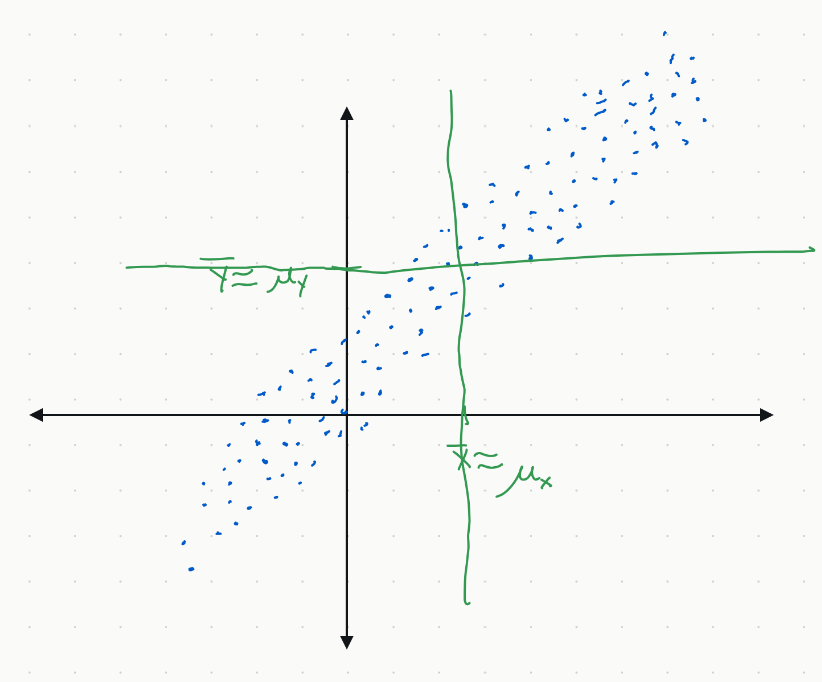
\includegraphics[width=0.6\textwidth]{associated-and-correlated}
	\caption{Exercise 5(a): Associated and correlated}
	\label{fig:associated-and-correlated}
\end{figure}

\easysubproblem{Give an example of two variables that are not correlated but are associated by drawing a plot.}\spc{7}

See Figure~\ref{fig:associated-not-correlated}.
\begin{figure}
	\centering
	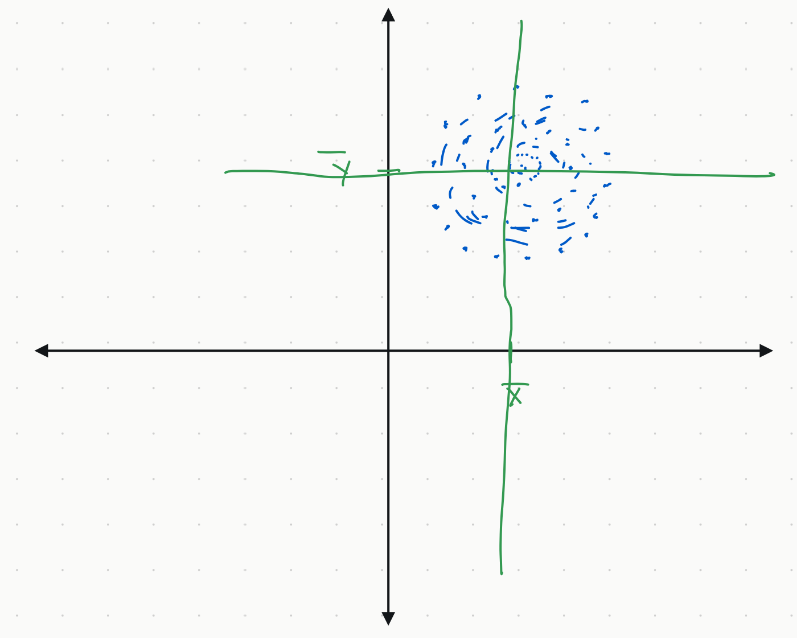
\includegraphics[width=0.6\textwidth]{associated-not-correlated}
	\caption{Exercise 5(b): Associated but not correlated}
	\label{fig:associated-not-correlated}
\end{figure}

\easysubproblem{Give an example of two variables that are not correlated nor associated by drawing a plot.}\spc{7}

See Figure~\ref{fig:not-associated-not-correlated}.
\begin{figure}
	\centering
	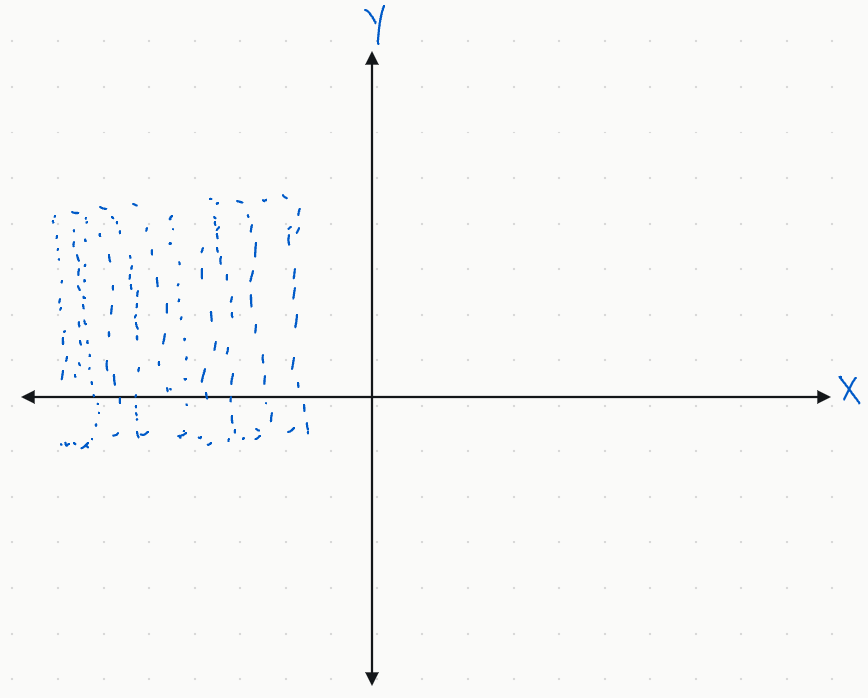
\includegraphics[width=0.6\textwidth]{not-associated-not-correlated}
	\caption{Exercise 5(c): Not associated and not correlated.}
	\label{fig:not-associated-not-correlated}
\end{figure}

\easysubproblem{Can two variables be correlated but not associated? Explain.}\spc{7}

No. If the variables are correlated, then as one increases, the other decreases (or increases). 
This suggests a relationship between the variables, and hence an association.

\end{enumerate}


\problem{These are questions about multivariate linear model fitting using the least squares algorithm.}

\begin{enumerate}

\hardsubproblem{Derive $\partialop{\c}{\c^\top A \c}$ where $\c \in \reals^n$ and $A \in \reals^{n \times n}$ but \textit{not} symmetric. Get as far as you can.}\spc{8}

Note that by the definition of matrix multiplication, the $k$th entry of $A\mathbf{c}$ is given by
\begin{align*}
	(A\mathbf{c})_k&=\sum_{j=1}^{n}a_{k,j}c_j
\end{align*}

Then
\begin{align*}
	\mathbf{c}^\top A\mathbf{c} &= \sum_{k=1}^{n}c_k\sum_{j=1}^{n}a_{k,j}c_j\\
	&=\sum_{k=1}^{n}\sum_{j=1}^{n}a_{k,j}c_kc_j
\end{align*}

To compute the vector derivative, we can focus on the partial derivative with
respect to the $c_i$

\begin{align*}
	\frac{\partial}{\partial c_i}[\mathbf{c}^\top A\mathbf{c}]
	&=\frac{\partial}{\partial c_i}
	\left[
	\sum_{k=1}^{n}\sum_{j=1}^{n}a_{k,j}c_kc_j
	\right]\\
	&=\sum_{k=1}^{n}\sum_{j=1}^{n}a_{k,j}\frac{\partial}{\partial c_i}[c_kc_j]\\
	&=\sum_{k=1}^{n}\sum_{j=1}^{n}a_{k,j}\left[c_j \frac{\partial}{\partial c_i}[c_k]
	+c_k\frac{\partial}{\partial c_i}[c_j] \right]\\
	&=\sum_{k=1}^{n}\sum_{j=1}^{n}a_{k,j}c_j\frac{\partial}{\partial c_i}[c_k]
	+\sum_{k=1}^{n}\sum_{j=1}^{n}a_{k,j}c_k\frac{\partial}{\partial c_i}[c_j]\\
	&=\sum_{j=1}a_{i,j}c_j+\sum_{k=1}^{n}a_{k,i}c_k
\end{align*}

Note that the evaluated to $0$ whenever $i\neq k$ in the first sum, and whenever
$i\neq j$ in the second sum. Now let's express this as a matrix multiplication:

\begin{align*}
	\frac{\partial}{\partial c_i}[\mathbf{c}^\top A \mathbf{c}]
	&=\sum_{j=1}a_{i,j}c_j+\sum_{k=1}^{n}a_{k,i}c_k\\
	&=A_{i,\cdot}\mathbf{c}+(A^\top)_{i,\cdot}\mathbf{c}
\end{align*}

Here, $A_{i,\cdot}$ denotes the $i$th row of $A$, and $(A^\top)_{i,\cdot}$ denotes the
$i$th row of $A^\top$. Now

\begin{align*}
	\frac{\partial}{\partial\mathbf{c}}[\mathbf{c}^\top A\mathbf{c}]
	&=\begin{bmatrix}
		\frac{\partial}{\partial c_1}[\mathbf{c}^\top A\mathbf{c}]\\
		\vdots\\
		\frac{\partial}{\partial c_n}[\mathbf{c}^\top A\mathbf{c}]
	\end{bmatrix}\\
	&=\begin{bmatrix}
		A_{1,\cdot}\mathbf{c}+(A^\top)_{1,\cdot}\mathbf{c}\\
		\vdots\\
		A_{n,\cdot}\mathbf{c}+(A^\top)_{n,\cdot}\mathbf{c}
	\end{bmatrix}\\
	&=\begin{bmatrix}
		A_{1,\cdot}\mathbf{c}\\
		\vdots\\
		A_{n,\cdot}\mathbf{c}
	\end{bmatrix}
	+\begin{bmatrix}
		(A^\top)_{1,\cdot}\mathbf{c}\\
		\vdots\\
		(A^\top)_{n,\cdot}\mathbf{c}
	\end{bmatrix}\\
	&=A\mathbf{c} + A^\top \mathbf{c}
\end{align*}

In the special case where $A$ is symmetric, we can see that we get $2A\mathbf{c}$.

\easysubproblem{Given matrix $X \in \reals^{n \times (p+1)}$, full rank and first column consisting of the $\onevec_n$ vector, rederive the least squares solution $\b$ (the vector of coefficients in the linear model shipped in the prediction function $g$). No need to rederive the facts about vector derivatives.}\spc{10}

We are assuming that the set of candidate functions $\mathcal{H}$ is the set of hyperplanes,
so we have a prediction function $g$ that can be used to predict $\hat{y}_i$ as follows:

\begin{align*}
	\hat{y}_i
	&=g(\mathbf{x}_i)\\
	&=w_0+w_1x_{i, 1}+\cdots+x_{i, p}\\
	&=\begin{bmatrix}
		1 & x_{i, 1} & \cdots & x_{i, p}
	\end{bmatrix}
	\begin{bmatrix}
		w_0\\
		w_1\\
		\vdots\\
		w_p
	\end{bmatrix}\\
	&=\mathbf{x}_i^\top \mathbf{w}
\end{align*}

Therefore, we can write the prediction vector as

\begin{align*}
	\hat{\mathbf{y}}
	:=\begin{bmatrix}
		\hat{y}_1\\
		\hat{y}_2\\
		\vdots\\
		\hat{y}_n
	\end{bmatrix}
	=\begin{bmatrix}
		\mathbf{x}_1^\top \mathbf{w}\\
		\mathbf{x}_2^\top \mathbf{w}\\
		\vdots\\
		\mathbf{x}_n^\top \mathbf{w}
	\end{bmatrix}
	=X\mathbf{w}
\end{align*}

The residual errors are given by $\mathbf{e}=\mathbf{y}-\hat{\mathbf{y}}$, and
hence the $SSE$ is given by

\begin{align*}
	SSE &= \sum_{i=1}^{n}e_i\\
	&=\mathbf{e}^\top\mathbf{e}\\
	&=(\mathbf{y}-\hat{\mathbf{y}})^\top (\mathbf{y}-\hat{\mathbf{y}})\\
	&=(\mathbf{y}^\top -\hat{\mathbf{y}}^\top)(\mathbf{y}-\hat{\mathbf{y}})
	\tag{Since $(A+B)^\top=A^\top+B^\top$}\\
	&=\mathbf{y}^\top \mathbf{y}-\mathbf{y}^\top \hat{\mathbf{y}}
	-\hat{\mathbf{y}}^\top \mathbf{y} + \hat{\mathbf{y}}^\top \hat{\mathbf{y}}\\
	&=\mathbf{y}^\top \mathbf{y}-\mathbf{y}^\top \hat{\mathbf{y}}
	-(\mathbf{y}^\top \hat{\mathbf{y}})^\top + \hat{\mathbf{y}}^\top \hat{\mathbf{y}}
	\tag{Since $(AB)^\top=B^\top A^\top$}\\
	&=\mathbf{y}^\top \mathbf{y}-2\mathbf{y}^\top \hat{\mathbf{y}}
	 + \hat{\mathbf{y}}^\top \hat{\mathbf{y}} \tag{Since $\mathbf{y}^\top \hat{\mathbf{y}}$ is a scalar}\\
	&=\mathbf{y}^\top\mathbf{y} - 2\mathbf{y}^\top X\mathbf{w}
	+ (X\mathbf{w})^\top (X\mathbf{w})\\
	&=\mathbf{y}^\top\mathbf{y} - 2 (X^\top \mathbf{y})^\top\mathbf{w}
	+ \mathbf{w}^\top X^\top (X\mathbf{w})
	\tag{Since $(AB)^\top=B^\top A^\top$}
\end{align*}

To minimize this quantity, we differentiate with respect to $\mathbf{w}$:

\begin{align*}
	\frac{\partial}{\partial \mathbf{w}}[SSE]
	&=\frac{\partial}{\partial \mathbf{w}}\left[
	\mathbf{y}^\top\mathbf{y} - 2 (X^\top \mathbf{y}^\top)^\top\mathbf{w}
	+ \mathbf{w}^\top X^\top (X\mathbf{w})
	\right]\\
	&=\frac{\partial}{\partial \mathbf{w}}[\mathbf{y}^\top\mathbf{y}]
	- 2  \frac{\partial}{\partial \mathbf{w}} [(X^\top \mathbf{y}^\top)^\top\mathbf{w}]
	+ \frac{\partial}{\partial \mathbf{w}} [\mathbf{w}^\top X^\top (X\mathbf{w})]\\
	&=\mathbf{0}_{p+1} - 2\cdot X^\top \mathbf{y} + 2\cdot X^\top X\mathbf{w}
\end{align*}

When we set this quantity to $\mathbf{0}_{p+1}$, we arrive at a vector $\mathbf{w}=\mathbf{b}$
that minimizes the $SSE$:
\begin{align*}
	\mathbf{0}_{p+1}&=\mathbf{0}_{p+1} - 2\cdot X^\top \mathbf{y} + 2\cdot X^\top X\mathbf{b}\\
	X^\top X\mathbf{b}&=X^\top \mathbf{y}\\
	\mathbf{b}&=(X^\top X)^{-1}X^\top \mathbf{y}
\end{align*}

provided that $X^\top X$ is invertible, or equivalently, that $\text{rank}[X^\top X]=p+1$.


\intermediatesubproblem{Consider the case where $p = 1$. Show that the solution for $\b$ you just derived in (b) is the same solution that we proved for simple regression. That is, the first element of $\b$ is the same as $b_0 = \ybar - r \frac{s_y}{s_x}\xbar$ and the second element of $\b$ is $b_1 = r \frac{s_y}{s_x}$.} \spc{7}

If $p=1$, then $X=\begin{bmatrix}
	\vec{\mathbf{1}}_n & \mathbf{x}_{\cdot, 1}
\end{bmatrix}$. We know that
\begin{align*}
	\mathbf{b} = (X^\top X)^{-1}X^\top\mathbf{y}
\end{align*}

Now
\begin{align*}
	X^\top \mathbf{y}
	&=\begin{bmatrix}
		1 & \cdots & 1\\
		x_1 & \cdots & x_n
	\end{bmatrix}
	\begin{bmatrix}
		y_1\\
		\vdots\\
		y_n
	\end{bmatrix}\\
	&=\begin{bmatrix}
		\sum_{i=1}^{n}y_i\\
		\sum_{i=1}^{n}x_iy_i
	\end{bmatrix}\\
	&=\begin{bmatrix}
		n\bar{y}\\
		\sum_{i=1}^{n}x_iy_i
	\end{bmatrix}
\end{align*}

Meanwhile,
\begin{align*}
	X^\top X
	&=\begin{bmatrix}
		1 & \cdots & 1\\
		x_1 & \cdots & x_n
	\end{bmatrix}
	\begin{bmatrix}
		1 & x_1\\
		\vdots & \vdots\\
		1 & x_n
	\end{bmatrix}\\
	&=\begin{bmatrix}
		n & \sum_{i=1}^{n}x_i\\
		\sum_{i=1}^{n}x_i & \sum_{i=1}^{n}x_i^2
	\end{bmatrix}\\
	&=\begin{bmatrix}
		n & n\bar{x}\\
		n\bar{x} & \sum_{i=1}^{n}x_i^2
	\end{bmatrix}
\end{align*}

Now we find the inverse of $X^\top X$:
\begin{align*}
	X^\top X
	&= \frac{1}{\text{det}(X^\top X)}
	\begin{bmatrix}
		\sum_{i=1}^{n}x_i^2 & -n\bar{x}\\
		-n\bar{x} & n
	\end{bmatrix}\\
	&=\frac{1}{n\cdot \sum_{i=1}^{n}x_i^2-n^2\bar{x}^2}
	\begin{bmatrix}
		\sum_{i=1}^{n}x_i^2 & -\bar{x}\\
		-\bar{x} & n
	\end{bmatrix}
\end{align*}

Now we multiply:
\begin{align*}
	\mathbf{b} &= (X^\top X)^{-1}(X^\top \mathbf{y})\\
	&=\frac{1}{n\cdot \sum_{i=1}^{n}x_i^2-n^2\bar{x}^2}
	\begin{bmatrix}
		\sum_{i=1}^{n}x_i^2 & -n\bar{x}\\
		-n\bar{x} & n
	\end{bmatrix}
	\begin{bmatrix}
		n\bar{y}\\
		\sum_{i=1}^{n}x_iy_i
	\end{bmatrix}\\
	&=\frac{1}{n\cdot \sum_{i=1}^{n}x_i^2-n^2\bar{x}^2}
	\begin{bmatrix}
		n\bar{y}\sum_{i=1}^{n}x_i^2-n\bar{x}\sum_{i=1}^{n}x_iy_i\\
		-n^2\bar{x}\bar{y}+n\sum_{i=1}^{n}x_iy_i
	\end{bmatrix}\\
	&=\frac{1}{ \sum_{i=1}^{n}x_i^2-n\bar{x}^2}
	\begin{bmatrix}
		\bar{y}\sum_{i=1}^{n}x_i^2-\bar{x}\sum_{i=1}^{n}x_iy_i\\
		-n\bar{x}\bar{y}+\sum_{i=1}^{n}x_iy_i
	\end{bmatrix}\\
\end{align*}

Hence we see that

\begin{align*}
	b_1 &= \frac{\sum_{i=1}^{n}x_iy_i-n\bar{x}\bar{y}}{ \sum_{i=1}^{n}x_i^2-\bar{x}^2}
\end{align*}

as before, and

\begin{align*}
	b_0 &= \frac{\bar{y}\sum_{i=1}^{n}x_i^2-\bar{x}\sum_{i=1}^{n}x_iy_i}{\sum_{i=1}^{n}x_i^2-n\bar{x}^2}\\
		&=\frac{\bar{y}\sum_{i=1}^{n}x_i^2}{\sum_{i=1}^{n}x_i^2-n\bar{x}^2}
	-\bar{x}\cdot \left(b_1 - \frac{n\bar{x}\bar{y}}{\sum_{i=1}^{n}x_i^2-n\bar{x}^2}\right)\\
	&=\frac{\bar{y}\cdot \left(\sum_{i=1}^{n}x_i^2-n\bar{x}^2\right)}{\sum_{i=1}^{n}x_i^2-n\bar{x}^2} - b_1\bar{x}\\
	&=\bar{y}-b_1\bar{x}
\end{align*}

Hence $b_0$ and $b_1$ are the same as when we did simple regression.

\easysubproblem{If $X$ is rank deficient, how can you solve for $\b$? Explain in English.} \spc{2}

The fact that $X$ is rank deficient implies that the columns of $X$ is linearly independent,
and hence, that some of the features are redundant. By eliminating the redundant features
from each observation $\mathbf{x}_i$, we can build a new matrix $X'$, which will have only
the non-redundant features, and will be full rank.

\hardsubproblem{Prove $\rank{X} =\rank{X^\top X}$.}\spc{9}

\begin{proof}
	Suppose $\mathbf{u}\in \text{null}(X)$. Then $X\mathbf{u}=\mathbf{0}_{n}$, and hence
	\begin{align*}
		(X^\top X)\mathbf{u}=X^\top(X\mathbf{u})=X^{\top}(\mathbf{0}_{n})=\mathbf{0}_{p+1}
	\end{align*}
	Hence, $\text{null}(X)\subseteq \text{null}(X^\top X)$. On the other hand,
	if $\mathbf{u}\in \text{null}(X^\top X)$, then $X^\top X\mathbf{u}=\mathbf{0}_{p+1}$,
	so
	\begin{align*}
		X^\top X\mathbf{u}&=\mathbf{0}_{p+1}\\
		\mathbf{u}^{\top}X^\top X\mathbf{u} &= 0\\
		(X \mathbf{u})^\top (X\mathbf{u})&=0\\
		\|X\mathbf{u}\|^2&=0
	\end{align*}
	The norm can only be zero if $X\mathbf{u}=\mathbf{0}_{n}$. Thus, we conclude
	that $\mathbf{u}\in\text{null}(X)$ and hence that $\text{null}(X^\top X)\subseteq \text{null}(X)$.
	With that, we can assert that $\dim \text{null}(X^\top X)=\dim\text{null}(X)$.
	Next, we use the Fundamental Theorem of Linear Maps (Rank-Nullity Theorem),
	applying it on both $X^\top X:\mathbb{R}^{p+1}\to\mathbb{R}^{p+1}$ and
	$X:\mathbb{R}^{p+1}\to\mathbb{R}^n$:
	\begin{align*}
		\dim\text{null}(X) + \dim\text{range}(X) = \dim\mathbb{R}^{p+1}=p+1\\
		\dim\text{null}(X^\top X) + \dim\text{range}(X^\top X) = \dim\mathbb{R}^{p+1}=p+1
	\end{align*}
	Subtracting the two equations and re-arranging, we arrive at
	$\dim\text{range}(X^\top X)=\dim\text{range}(X)$. Since the dimension of
	the range is precisely the rank, we are done.
\end{proof}

%\hardsubproblem{Given matrix $X \in \reals^{n \times (p+1)}$, full rank and first column consisting of the $\onevec_n$ vector, now consider cost multiples (\qu{weights}) $c_1, c_2, \ldots, c_n$ for each mistake $e_i$. As an example, previously the mistake for the 17th observation was $e_{17} := y_{17} - \hat{y}_{17}$ but now it would be $e_{17} := c_{17} (y_{17} - \hat{y}_{17})$.  Derive the weighted least squares solution $\b$. No need to rederive the facts about vector derivatives. Hints: (1) show that SSE is a quadratic form with the matrix $C$ in the middle (2) Split this matrix up into two pieces i.e. $C = C^{\half} C^{\half}$, distribute and then foil (3) note that a scalar value equals its own transpose and (4) use the vector derivative formulas.}\spc{10}


\intermediatesubproblem{[MA] If $p=1$, prove $r^2 = R^2$ i.e. the linear correlation is the same as proportion of sample variance explained in a least squares linear model.}\spc{6}



\intermediatesubproblem{Prove that $g(\bracks{1 ~\xbar_1~ \xbar_2~ \ldots~ \xbar_p}) =\bar{y}$ in OLS.}\spc{7}

\begin{proof}
	\begin{align*}
		g(\begin{bmatrix}
			1 & \bar{x}_1 & \bar{x}_2 & \cdots & \bar{x}_p
		\end{bmatrix})
		&=\begin{bmatrix}
			1 & \bar{x}_1 & \bar{x}_2 & \cdots & \bar{x}_p
		\end{bmatrix}
		\mathbf{b}\\
		&=\begin{bmatrix}
			\frac{1}{n}\sum_{i=1}^{n}1 & \frac{1}{n}\sum_{i=1}^{n}x_{i,1}
			& \frac{1}{n}\sum_{i=1}^{n}x_{i,2}
			& \cdots
			& \frac{1}{n}\sum_{i=1}^{n}x_{i,p}
		\end{bmatrix}\mathbf{b}\\
		&=\left(\frac{1}{n}\vec{\mathbf{1}}^\top X\right)\mathbf{b}\\
		&=\left(\frac{1}{n}\vec{\mathbf{1}}^\top X\right)(X^\top X)^{-1}X^\top \mathbf{y}
		\tag{by definition of $\mathbf{b}$}\\
		&=\frac{1}{n}\vec{\mathbf{1}}^\top H\mathbf{y}
		\tag{by definition of $H$}\\
		&=\frac{1}{n}(H^\top \vec{\mathbf{1}})^\top\mathbf{y}
		\tag{since $(AB)^\top B^\top A^\top$}\\
		&=\frac{1}{n}(H\vec{\mathbf{1}})^\top \mathbf{y}
		\tag{$H=H^\top$}\\
		&=\frac{1}{n}(\vec{\mathbf{1}}^\top)\mathbf{y}
		\tag{$\vec{\mathbf{1}}\in co\ell [X]$}\\
		&=\bar{y}
	\end{align*}
\end{proof}

\intermediatesubproblem{Prove that $\bar{e} = 0$ in OLS.}\spc{10}

\begin{proof}
	\begin{align*}
		\sum_{i=1}^{n}e_i
		&=\sum_{i=1}^{n}(y_i-\hat{y}_i)\\
		&=\sum_{i=1}^{n}1\cdot (y_i-\hat{y}_i)\\
		&=\vec{\mathbf{1}}_n^\top(\mathbf{y}-\hat{\mathbf{y}})\\
		&=\vec{\mathbf{1}}_n^\top (\mathbf{y}-H \mathbf{y})\\
		&=\vec{\mathbf{1}}_n^\top(I-H)\mathbf{y}\\
		&=[(I-H)^\top \mathbf{1}]^\top\mathbf{y}\\
		&=[(I-H)\vec{\mathbf{1}}_n]^\top \mathbf{y}
		\tag{$I$ and $H$ are symmetric}\\
		&=[\mathbf{0}_n]^\top \mathbf{y}\\
		&=0
	\end{align*}
	Note that $(I-H)$ is an orthogonal projection matrix onto $co\ell [X]^\top$,
	the orthogonal complement of the column space of $X$. Since $\vec{\mathbf{1}}$ belongs
	to the column space of $X$, the orthogonal projection matrix $I-H$ maps it to $\mathbf{0}_n$.
	Now $\bar{e}=\frac{1}{n}\sum_{i=1}^{n}e_i=0$.
\end{proof}

\hardsubproblem{If you model $\y$ with one categorical nominal variable that has levels $A, B, C$, prove that the OLS estimates look like $\ybar_A$ if $x = A$, $\ybar_B$ if $x = B$ and $\ybar_C$ if $x = C$. You can choose to use an intercept or not. Likely without is easier.}\spc{10}

\begin{proof}
	Without an intercept, the matrix $X$ is
	\begin{align*}
		X &= \begin{bmatrix}
			1 & 0 & 0\\
			\vdots & \vdots & \vdots\\
			1 & 0 & 0\\
			0 & 1 & 0\\
			\vdots & \vdots & \vdots\\
			0 & 1 & 0 \\
			0 & 0 & 1\\
			\vdots & \vdots & \vdots\\
			0 & 0 & 1
		\end{bmatrix}
		=\begin{bmatrix}
			\mathbf{x}_{\cdot, A} & \mathbf{x}_{\cdot, B} & \mathbf{x}_{\cdot, C}
		\end{bmatrix}
	\end{align*}
	The first column ($\mathbf{x}_{\cdot, A}$) corresponds to inputs where $x=A$,
	the second column ($\mathbf{x}_{\cdot, B}$) to inputs where $x=B$, and the third
	column ($\mathbf{x}_{\cdot, C}$)to inputs where $x=C$. The least square estimate
	is given by
	\begin{align*}
		\mathbf{b}=(X^\top X)^{-1}X^\top \mathbf{y}
	\end{align*}
	We need to compute the vector, so we will do it in parts:
	\begin{align*}
		X^\top \mathbf{y}
		&=\begin{bmatrix}
			\mathbf{x}_{\cdot, A}^\top\\
			\mathbf{x}_{\cdot, B}^\top\\
			\mathbf{x}_{\cdot C}^\top
		\end{bmatrix}
		\mathbf{y}
		=\begin{bmatrix}
			\mathbf{x}_{\cdot, A}^\top\mathbf{y}\\
			\mathbf{x}_{\cdot, B}^\top\mathbf{y} \\
			\mathbf{x}_{\cdot C}^\top\mathbf{y}
		\end{bmatrix}
		=\begin{bmatrix}
			\sum_{ \{\, i \mid x_i=A\} }y_i\\
			\sum_{ \{\, i \mid x_i=B\} }y_i\\
			\sum_{ \{\, i \mid x_i=C\} }y_i
		\end{bmatrix}\\
		&=\begin{bmatrix}
			n_A\bar{y}_A\\
			n_B\bar{y}_B\\
			n_C\bar{y}_C
		\end{bmatrix}
	\end{align*}
	Notice that since the vector $\mathbf{y}$ of responses corresponds to the inputs,
	the values line up to give, for example, $n_A\bar{y}_A$ (where $n_A$ is the
	number of entries where $x=A$). Next we must compute $X^\top X$:
	\begin{align*}
		X^\top X &=\begin{bmatrix}
			\mathbf{x}_{\cdot, A}^\top \mathbf{x}_{\cdot, A} & \mathbf{x}_A^\top \mathbf{x}_{\cdot, B} & \mathbf{x}_A^\top \mathbf{x}_{\cdot, C}\\
			\mathbf{x}_{\cdot, B}^\top \mathbf{x}_{\cdot, A} & \mathbf{x}_{\cdot, B}^\top \mathbf{x}_{\cdot, B} & \mathbf{x}_{\cdot, B}^\top \mathbf{x}_{\cdot, C}\\
			\mathbf{x}_{\cdot, C}^\top \mathbf{x}_{\cdot, A} & \mathbf{x}_{\cdot, C}^\top \mathbf{x}_{\cdot, B} & \mathbf{x}_{\cdot, C}^\top \mathbf{x}_{\cdot, C}
		\end{bmatrix}
		=\begin{bmatrix}
			n_A & 0 & 0\\
			0 & n_B & 0\\
			0 & 0 & n_C
		\end{bmatrix}
	\end{align*}
	Since the matrix is diagonal, the inverse is easy to compute:
	\begin{align*}
		(X^{T}X)^{-1}&=\begin{bmatrix}
			\frac{1}{n_A} & 0 & 0\\
			0 & \frac{1}{n_B} & 0\\
			0 & 0 & \frac{1}{n_C}
		\end{bmatrix}
	\end{align*}
	Now we can compute the least square estimate:
	\begin{align*}
		\mathbf{b}
		&=(X^\top X)^{-1}X^\top \mathbf{y}\\
		&=\begin{bmatrix}
			\frac{1}{n_A} & 0 & 0\\
			0 & \frac{1}{n_B} & 0\\
			0 & 0 & \frac{1}{n_C}
		\end{bmatrix}
		\begin{bmatrix}
			n_A\bar{y}_A\\
			n_B\bar{y}_B\\
			n_C\bar{y}_C
		\end{bmatrix}
		=\begin{bmatrix}
			\bar{y}_A\\
			\bar{y}_B\\
			\bar{y}_C
		\end{bmatrix}
	\end{align*}
	The prediction is given by $g(\mathbf{x})=\mathbf{x}^\top \mathbf{b}$,
	so we can proceed to compute the predictions of interest. Note that
	if $x=A$, then the input is $\begin{bmatrix}
		1 & 0 & 0
	\end{bmatrix}^\top$. In particular, only one entry is $1$ at a time.
	Finally,
	\begin{align*}
		g\left(\begin{bmatrix}
			1 & 0 & 0
		\end{bmatrix}^\top\right)
		&=\begin{bmatrix}
			1 & 0 & 0
		\end{bmatrix}
		\mathbf{b}\\
		&=\begin{bmatrix}
			1 & 0 & 0
		\end{bmatrix}
		\begin{bmatrix}
			\bar{y}_A\\
			\bar{y}_B\\
			\bar{y}_C
		\end{bmatrix}\\
		&=\bar{y}_A
	\end{align*}
	A similar calculations shows that $g$ predicts $\bar{y}_B$ and $\bar{y}_C$ for
	$x=B$ and $x=C$, respectively.
\end{proof}

\intermediatesubproblem{[MA] Prove that the OLS model always has $R^2 \in \zeroonecl$.}\spc{5}

\begin{proof}
	First compute the mean-control response:
	\begin{align*}
		\underset{co\ell [X]}{\text{proj}}(\mathbf{y}-\bar{y}\cdot \vec{\mathbf{1}}_n)
		&=(\mathbf{y}-\bar{y}\cdot \vec{\mathbf{1}}_n)\\
		&=H\mathbf{y}-\bar{y} H\vec{\mathbf{1}}_n\\
		&=\hat{\mathbf{y}} - \bar{y} \cdot \vec{\mathbf{1}}_n
		\tag{since $\vec{\mathbf{1}}\in co\ell[X]$}
	\end{align*}
	Moreover,
	\begin{align*}
		(\mathbf{y}-\bar{y}\vec{\mathbf{1}}_n)-(\hat{\mathbf{y}}-\bar{y}\vec{\mathbf{1}}_n)
		=\mathbf{y}-\hat{\mathbf{y}}
		=\mathbf{e}
	\end{align*}
	In particular, since $\mathbf{e}$ is orthogonal to the column space of $X$,
	and $\hat{\mathbf{y}}-\bar{y}\vec{\mathbf{1}}_n$ belongs to the column space of $X$
	(it is a linear combination of such vectors), it follows that
	$\hat{\mathbf{y}}-\bar{y}\vec{\mathbf{1}}_n$ and $\mathbf{e}$ are orthogonal.
	Therefore, we can apply the Pythagorean Theorem to write
	\begin{align*}
		\|\mathbf{y}-\bar{y}\vec{\mathbf{1}}_n\|^2
		&=\|\hat{\mathbf{y}}-\bar{y}\vec{\mathbf{1}}_n\|^2 + \|\mathbf{e}\|^2\\
		\sum_{i=1}^{n}(y_i-\bar{y})^2 &=
		\sum_{i=1}^{n}(\hat{y_i}-\bar{y})^2+\sum_{i=1}^{n}e_i^2\\
		SST &= SSR + SSE
	\end{align*}
	Now using trigonometry, we find that
	\begin{align*}
		\cos\theta^2 &= \frac{\|\hat{\mathbf{y}}-\bar{y}\vec{\mathbf{1}}_n\|^2}{\|\mathbf{y}-\bar{y}\vec{\mathbf{1}}_n\|^2}\\
		&=\frac{SST-SSE}{SST}\\
		&=1-\frac{SSE}{SST}\\
		&=R^2
	\end{align*}
	Finally, since $\cos\theta^2\in[0, 1]$, it follows that $R^2\in[0, 1]$.
\end{proof}

\end{enumerate}



\end{document}

